%%% File encoding is ISO-8859-1 (also known as Latin-1)
%%% You can use special characters just like �,? and �
%%% LaTeX template by Manuel Kuehner, 2015

%%% If you use this template then please give credit like this:
%%% ----------------------------
% LaTeX code inspired by the LaTeX Thesis Template by Manuel Kuehner 
% www.bedienhaptik.de/latex-template/
%%% ----------------------------

% ##############################################
% Start: Template Preamble
% ##############################################
%

% Documentclass definition
%%% File encoding is ISO-8859-1 (also known as Latin-1)
%%% You can use special characters just like �,� and �

% KOMA-Script class 'scrbook'
% Link to the documentation: 
% German: http://mirrors.ctan.org/macros/latex/contrib/koma-script/doc/scrguide.pdf
% English: http://mirrors.ctan.org/macros/latex/contrib/koma-script/doc/scrguien.pdf
% CTAN: http://www.ctan.org/pkg/koma-script
% Author of the KOMA-Script family is Markus Kohm
\documentclass%
[%
paper=a4
,fontsize=11pt % common are 10, 11 or 12
,headings=big
,parskip
,numbers=noendperiod % 2.3.1 vs 2.3.1. (no dot after the last chapter number)
,twoside=true
,toc=bibliography % Bibliography appears in Table of Contents (without a number)
,toc=listof % List of Figures and List of Tables appear in Table of Contents
,version=last % Use latest version of the KOMA-Script
]%
{scrbook}

% Loading additional packages from the KOMA-Script family
%%% File encoding is ISO-8859-1 (also known as Latin-1)
%%% You can use special characters just like �,� and �


\usepackage{scrhack}

% Better support for marginnotes
% new command: \marginnote
% LaTeX standard command: \marginpar
% CTAN: http://www.ctan.org/pkg/marginnote
\usepackage{marginnote}

% Extended header and footer support
% CTAN: http://www.ctan.org/pkg/scrpage2
\usepackage[%
  	automark
  	,ilines
	,headsepline
	,footsepline
]{scrpage2}

% Page layout definition
%%% File encoding is ISO-8859-1 (also known as Latin-1)
%%% You can use special characters just like �,� and �

% User friendly interface to change layout parameters
% CTAN: http://www.ctan.org/pkg/geometry
\usepackage{geometry}
\geometry{% siehe geometry.pdf (Figure 1)
	bottom=30mm,
	showframe=false, % For debugging: try true and see the layout frames
	margin=30mm,
	marginparsep=3mm,
	marginparwidth=20mm
}

% Standard packages
%%% File encoding is ISO-8859-1 (also known as Latin-1)
%%% You can use special characters just like �,� and �

% Input encoding is 'latin1' (Latin 1 - also known as ISO-8859-1)
% CTAN: http://www.ctan.org/pkg/inputenc
% 
% A newer package is available - you may look into:
% \usepackage[x-iso-8859-1]{inputenc}
% CTAN: http://www.ctan.org/pkg/inputenx
\usepackage[latin1]{inputenc}

% Font Encoding is 'T1' -- important for special characters such as Umlaute � or � and special characters like � (enje)
% CTAN: http://www.ctan.org/pkg/fontenc
\usepackage[T1]{fontenc}

% Language support for 'english' (alternative 'ngerman' or 'french' for example)
% CTAN: http://www.ctan.org/pkg/babel
\usepackage[english]{babel} 

% Doing calculations with LaTeX units -- needed for the vertical line in the footer
% CTAN: http://www.ctan.org/pkg/calc
\usepackage{calc}

% Extended graphics support 
% There is also a package named 'graphics' - watch out!
% CTAN: http://www.ctan.org/pkg/graphicx
\usepackage{graphicx}

% Extendes support for floating objects (tables, figures), adds the [H] placing option (\begin{figure}[H]) which palces it "Here" (without any doubt).
% CTAN: http://www.ctan.org/pkg/float
\usepackage{float}

% Extended color support
% I use the command \definecolor for example. 
% Option 'Table': Load the colortbl package, in order to use the tools for coloring rows, columns, and cells within tables.
% CTAN: http://www.ctan.org/pkg/xcolor
\usepackage[table]{xcolor} 

% Nice tables
% CTAN: http://www.ctan.org/pkg/booktabs
\usepackage{booktabs}

% Better support for ragged left and right. Provides the commands \RaggedRight and \RaggedLeft. 
% Standard LaTeX commands are \raggedright and \raggedleft
% http://www.ctan.org/pkg/ragged2e
\usepackage{ragged2e}

% Create function plots directly in LaTeX
% CTAN: http://www.ctan.org/pkg/pgfplots
\usepackage{pgfplots}
\pgfplotsset{compat=1.11}

\usepackage{subfigure}

% ####-Important-####
%
% Definition of the two main colors
% -----------------------
% The corresponding xcolor package ist loaded in the file 
% 01_Preamble/StandardPackages.tex
%
% ####-Important-####
\definecolor[named]{myColorMainA}{RGB}{0,26,153}
\definecolor[named]{myColorMainB}{RGB}{174,49,54}

% Customization of 
% - Floating Objects (Caption) 
% - Table of Contents (TOC)
% - List of Figures
% - List of Tables
% - Headings (like chapter, section, etc.)
%%% File encoding is ISO-8859-1 (also known as Latin-1)
%%% You can use special characters just like �,� and �

% ##############################################
% Start: Table of Contents (TOC) Customization
% ##############################################
%

% Level for numbered captions
\setcounter{secnumdepth}{5}

% Level of chapters that appear in Table of Contents
\setcounter{tocdepth}{5} % bis wohin ins Inhaltsverzeichnis aufnehmen
% -2 no caption at all
% -1 part
% 0  chapter
% 1  section    
% 2  subsection 
% 3  subsubsection
% 4  paragraph
% 5  subparagraph

% KOMA-Script code to adjust TOC
% Applying the color 'myColorMainA' which is defined in the main file (MainFile.tex)
\makeatletter
\addtokomafont{chapterentrypagenumber}{\color{myColorMainA}}
\addtokomafont{chapterentry}{\color{myColorMainA}}
\makeatother

%
% #######################
% End: Table of Contents (TOC) Customization
% #######################

% ##############################################
% Start: Floating Object Customization
% ##############################################
%

% Extended support for catioons of figures and tables etc.
% CTAN: http://www.ctan.org/pkg/caption
\usepackage[%
	font={small},
	labelfont={bf,sf},
	format=hang, % try plain or hang
	margin=5pt,
]{caption}
%

% #######################
% End: Floating Object Customization
% #######################

% ##############################################
% Start: Headings Customization
% ##############################################
%

% KOMA-Script code to customize the headings
% Applying the color 'myColorMainA' which is defined in the main file (MainFile.tex)
\addtokomafont{chapter}{\color{myColorMainA}}
\addtokomafont{section}{\color{myColorMainA}}
\addtokomafont{subsection}{\color{myColorMainA}}
\addtokomafont{subsubsection}{\color{myColorMainA}}
\addtokomafont{paragraph}{\color{myColorMainA}}
\addtokomafont{subparagraph}{\color{myColorMainA}}

% #######################
% End: Headings Customization
% #######################


% Customization of the header, footer and teh margin note
%%% File encoding is ISO-8859-1 (also known as Latin-1)
%%% You can use special characters just like �,� and �

% Custom command fpr the margin notes: \myMarginnote{Your Text}
% Comment on the \lineskiplimit=-\maxdimen:
% See http://tex.stackexchange.com/questions/49072/
% Without it the line spacing of the normal text was changed (ugly).
\newcommand{\myMarginnote}[1]{%
	\marginnote{% needs marginnote package
		\ifthispageodd{\RaggedRight}{\RaggedLeft}% needs ragged2e package
		\color{myColorMainB}%
		\lineskiplimit=-\maxdimen% 
		\normalfont\sffamily\scriptsize%
		#1}%
}

% ##############################################
% Start: Header and Footer Customization
% ##############################################
%

% KOMA-Script code for header and footer font
\setkomafont{pageheadfoot}{%
	\normalfont\sffamily\bfseries
	}
\setkomafont{pagefoot}{%
	\normalfont\sffamily
	}
\setkomafont{pagenumber}{%
	\normalfont\rmfamily
	}

% Define width of header
\setheadwidth[0pt]{textwithmarginpar}

% Define with of header line
\setheadsepline{0.4pt}

% Define width of footer
\setfootwidth[0pt]{text}
% Define with of footer line (here: no line)
\setfootsepline[text]{0pt}

% Some calculations
% calc package is needed which is loaded here: 01_Preamble/CommonPackages.tex
% If you want to understand the calculations visit:
% http://en.wikibooks.org/wiki/LaTeX/Page_Layout
\newlength{\myLenghthFootAbstand}
\setlength{\myLenghthFootAbstand}{\paperheight-1in-\topmargin- \headheight-\headsep-\textheight-\footskip}
\newlength{\myLenghthTemp}
\setlength{\myLenghthTemp}{\myLenghthFootAbstand+\baselineskip}

% Define content of header and footer
% Using some scrpage2 commands here. The scrpage2 package is loaded here: 01_Preamble/KOMA-Script-Packages.tex
% Some LaTeX magic...
% Clear all defaults
\clearscrheadfoot
% Header
\ohead{%
	\textcolor{myColorMainA}{\headmark}
	}
% Left (even page numbers) footer
\lefoot%
[% scrplain style (begin)
	\setlength{\unitlength}{\myLenghthFootAbstand}%
	\begin{picture}(0,0)%
		\put(0,-1)%
		{%
			\makebox(0,0)[lb]%
			{%
				\rule{0.4pt}{\myLenghthTemp}%
			}%
		}%
	\end{picture}\llap{\pagemark~}%
]% scrplain style (end)
%
{% scrheadings style (begin)
	\setlength{\unitlength}{\myLenghthFootAbstand}%
	\begin{picture}(0,0)%
		\put(0,-1)%
		{%
			\makebox(0,0)[lb]%
			{%
				\rule{0.4pt}{\myLenghthTemp}%
			}%
		}%
	\end{picture}\llap{\pagemark~}%
}% scrheadings style (end)

% Right (odd page numbers) footer
\rofoot%
[% scrplain style (begin)
	\rlap{~\pagemark}%%
	\setlength{\unitlength}{\myLenghthFootAbstand}%
	\begin{picture}(0,0)%
		\put(0,-1)%
		{%
			\makebox(0,0)[lb]%
			{%
				\rule{0.4pt}{\myLenghthTemp}%
			}%
		}%
	\end{picture}%
]% scrplain style (end)
%
{% scrplain style (begin)
	\rlap{~\pagemark}%%
	\setlength{\unitlength}{\myLenghthFootAbstand}%
	\begin{picture}(0,0)%
		\put(0,-1)%
		{%
			\makebox(0,0)[lb]%
			{%
				\rule{0.4pt}{\myLenghthTemp}%
			}%
		}%
	\end{picture}%
}% scrplain style (end)

%
% #######################
% End: Header and Footer Customization
% #######################

% Optimize paragraphs (avoid overfull... warnings)
%%% File encoding is ISO-8859-1 (also known as Latin-1)
%%% You can use special characters just like �,� and �

% This is an suggestion from Axel Reichert (LaTeX package author)
% See CTAN: http://www.ctan.org/author/reichert
% See CTAN: http://www.ctan.org/pkg/l2tabu-english (Cgapter: 1.8 Should I use \sloppy?)

\tolerance 1414
\hbadness 1414
\emergencystretch 1.5em
\hfuzz 0.3pt
\widowpenalty=10000
\vfuzz \hfuzz
\raggedbottom

% PDF related packages

\usepackage[%
bookmarks, % Create bookmarks
bookmarksopen=true, % Unfold bookmatk tree in PDF viewer when document is opened
bookmarksopenlevel=1, % Level of unfolding
bookmarksnumbered=true, % Number bookmarks
hidelinks, % do not highlight hyperlinks -- looks ugly
% Ansicht beim �ffnen
pdfpagelabels=true, % See manual...
plainpages=false, % See manual...
hyperfootnotes=true, % Hyperlinks for footnotes
hyperindex=true, % Indexeintr�age verweisen auf Text
]{hyperref}

% PDF related packages

\usepackage[]{blindtext}
% The custom command \myMarginnote is defined in the file: 
% 01_Preamble/HeaderFooterMarginnote.tex
\renewcommand{\blindmarkup}[1]{\myMarginnote{#1}}

%
% #######################
% Ende: Template Preamble
% #######################

% ##############################################
% Start: Document
% ##############################################
%
% ------------------------------------------------------------------
\begin{document}

% Title page
%%% File encoding is ISO-8859-1 (also known as Latin-1)
%%% You can use special characters just like �,� and �

% Title page using \maketitle (a more flexible alternative is the titlepage environment)
\title{The Smoking Gun: The Inside-Out Quenching of the red spiral galaxy UGC11680 }
%\subtitle{Jeffrey}
\author{Jeffrey E. Barcenas Mosqueda}
\date{12.01.2016}
\maketitle
% Empty page after title page
\cleardoublepage

% Activate header and footer defined in the file:
% 01_Preamble/HeaderFooterMarginnote.tex
\pagestyle{scrheadings}

% Activate roman numbering (e. g. xii)	
\pagenumbering{roman}

% Start with page 1 (I)
\setcounter{page}{1}

% Prologue

% Chapter without numbering but with appearance in the Table of Contents
% \addchap is a command from KOMA-Script
\addchap{Prologue}

\Blindtext[3][1]

% Abstract
%%% File encoding is ISO-8859-1 (also known as Latin-1)
%%% You can use special characters just like �,� and �

% Chapter without numbering but with appearance in the Table of Contents
% \addchap is a command from KOMA-Script
\addchap{Abstract}

\Blindtext[2][2]

\blindtext

% Table of Contents and Lost of Figures/Tables
%%% File encoding is ISO-8859-1 (also known as Latin-1)
%%% You can use special characters just like �,� and �

% Table of Contents (TOC)
% Special code so that it appears as a bookmark in the PDF viewer
\phantomsection
\pdfbookmark[0]{Table of Contents}{toc} % <-- Please edit the name if you want a different text as a bookbarl for the Table of Contents
\tableofcontents
% List of Figures
\listoffigures
% List of Tables
\listoftables 

% Activate arabic numbering (e. g. 12)	
\pagenumbering{arabic}

% Start with page 1
\setcounter{page}{1}

% Introduction
%%% File encoding is ISO-8859-1 (also known as Latin-1)
%%% You can use special characters just like �,� and �

\chapter{Introduction}

Why UGC11680NED01 spiral galaxy is red? 

With this simple question began work presented in this thesis.

In any textbook we learn that elliptical galaxies are red and spiral galaxies are blue, Two morphologies, two colors. 
We can distinguish between these types of galaxies without really studying very thoroughly, and go with something else.
However, not everything is so easy, people have discovered red spiral galaxies (Bundy) in the local universe. 
This simplification is justified because most galaxies follow a relationship strictest Color-morphology.
To study the nature of the red spiral, we will have many preconception off on their star formation. 
This has certain advantages in the analysis. Thus we will take the spiral of the catalog, and try to analyze their stellar populations.

The advent of large galaxy surveys like the Sloan Digital Sky
Survey (SDSS) in which photometry (and therefore color) is
readily available to millions of objects has led to
use of optical colors to define "early" galaxies "tardias``
(Eg Cooray 2005; Bundy et al 2006 ;. Croton Lee et al 2007 ;.
And pen 2007; Salimbeni et al. 2008; Simon et al. 2009). This method
is particularly favored because obtaining morphologies for a large
number of galaxies has been impossible until recently. This simplification
is justified because it has been shown many times that
Most galaxies follow a color ratio - strict morphology.
For example, Mignoli et al. (2009) showed that 85 percent of
galaxies to $ z \ approx $ 1 are either, red galaxies dominated by its bulb or
blue galaxies dominated by its disc; while Conselice (2006) showed
Similar result 22 000 galaxies of low redshift (both using automated
methods for morphological classification).
However, the clear correlation between the color and morphology
surprising given that the colors of the galaxies are determined primarily
for its stellar content (and therefore their recent star formation,
especially within the last Gyr), while morphology is mainly
driven by the dynamic history. The clear link between color
and morphology gives a strong indication that the time scales
and the processes that drive morphological transformation and
cessation of star formation are related (at least in most
cases). In this paper, however, we consider a class of object (red spiral)
where it seems that the relationship described above seems to be fulfilled.

Since the morphology-density relation quantified first
(Dressler, 1980), many mechanisms have been proposed for
Blue transformation, disk galaxies forming stars at low density
regions of the Universe, a, passive red galaxies in clusters first type.
A recent review of many of the proposed mechanisms and
the evidence supporting them, can be found at Boselli and Gavazzi
(2006). Clearly two things must happen for a blue star-forming spiral
Galaxy becomes a passive early red type. Education First Star
You must cease (which can alter the morphology indirectly cause
spiral arms and the disc generally disappear, possibly producing a
S0 lenticular or a spiral). Secondly, in order to produce a bona
fide elliptical, the same or a different process must also dynamically
alter the stellar kinematics of the galaxy.

The presence of an unusual red colored or passive (ie, not forming star)
population of spiral galaxies in clusters of galaxies was first
said Van den Bergh (1976) in the Virgo cluster. later studies
distant cluster of galaxies in the Hubble Space Telescope (HST)
images also revealed a number of so-called "passive"
spiral galaxies with a lack of ongoing star formation (Couch et al.
1998; Dressler et al. 1,999; Poggianti et al. 1,999). Passive delayed type
galaxies were identified on the move to lower red outside SDSS
clusters of Goto et al. (2003) using the concentration as a proxy for
morphology. Spirals liabilities of a cluster at z ~ 0.4 were studied by
Moran et al. (2006) who found stories of star formation in the Galaxy Evolution Explorer (GALEX) consistent with observations
closing of star formation choke (as described
by Bekki, sofa and Shioya 2002). Spirals liabilities have also revealed
in a cluster at z ~ 0.1 in the A9012 / Galaxy Space Telescope
Evolution Survey (STAGES) using HST morphologies Wolf et al.
Spectral energy distributions (2009), rest-frame near-ultraviolet optical
(SED; Wolf, Gray \& Meisenheimer 2005) and data from 24 microns
Spitzer (Gallazzi et al. 2009). In this series of papers, 'dusty
are red late types "and" optically passive final rates "to be
largely the same, with a non-zero (but reduced significantly)
rate of star formation revealed by infrared data.
Spiral red / final year types have been studied in several recent articles
(Lee et al 2008 ;. Cortese and Hughes 2009; Deng et al 2009 ;. Hughes
And Cortese 2009) and Mahajan and Raychaudhury (2009) who
speak passive blue galaxies (ie, galaxies with blue, but
showing signs of recent star formation in their spectra)
most of which seem to have late-type morphologies and have very
Recently off star formation. These could be the progenitors
red spirals. Bundy et al. (2010) studied the redshift
evolution of disk galaxies red string as components in the
Cosmic Evolution Survey (COSMOS) and use it to estimate that
up to 60 percent of spiral galaxies must go through this
phase on the way to the red string - making it an important
evolutionary step.

It is clear that all spiral galaxies can be affected by various physical
processes as they evolve - in this paper seeks to identify
that they are most important for red spirals, asking how are
able to shut down star formation, keeping their spiral morphology.
A list of possible mechanisms include processes
It will depend on the environment. (1) galaxy-galaxy interactions: high density
regions, there is a greater probability of interaction
with other galaxies. Most major mergers destroy spiral structure
(Toomre and Toomre 1972) unless they involve parents in rich gas
(Hopkins et al. 2009), but some interactions can be quite
soft (for example, Walker and Hernquist Mihos 1996), for example minormergers,
tidal interactions, etc. (2) The interaction with the cluster itself
also it produced and can be removed form the gas reservoir
star formation. This may be due to tidal effects (eg Gnedin 2003)
or interaction with the intercluster hot gas, either through thermal evaporation (Cowie and Songaila 1977) or ram pressure extraction
(Gunn and Gott 1972). (3) The processes as harassment (Moore et al.
1999) and the starvation and strangulation (Larson, Tinsley and Caldwell
1,980; Bekki et al. 2002) have also shown to have a significant
cant effect in late-type galaxies. Harassment refers to heating
gas for many small interactions, while hunger or strangulation
It refers to the gradual depletion of disk after the hot gas has halo
It has been stripped away. Both of these mechanisms occur in much greater
radios cluster (ie, lower densities) than the "classic environmental effects.
Internal mechanisms may be more important. For instance,
(4) the last semi-analytic models of galaxy formation invoke all
feedback from a massive black hole active center [or galactic nuclei
(AGN)] to explain the most massive elliptical galaxies red (Granato
et al. 2004; Silk 2005; Schawinski et al. 2006; Croton et al. 2006;
Bower et al. 2,006), although the effect of this process on disk galaxies
has been studied less, you can still have some effect (Okamoto,
Nemmen and Bower 2008). (5) Another cause could be the instability bar
in spiral galaxies that lead the gas into (eg Combes
Sanders 1981), and may trigger the AGN activity and / or central star
training (eg Shlosman, Peletier and Knapen 2000), perhaps using
the gas reservoir in the outer disk and spirals making red. (6)
Finally, spirals Red spirals could simply be old who have exhausted
all its gas in normal star-forming activities without any
basic interaction. In normal spirals, gas supplying current
star formation comes from material falling from a reservoir in the
outer halo (Boselli and Gavazzi 2006). As first it suggested by Larson,
Tinsley and Caldwell (1980) and expanded by Bekki et al. (2002),
extracting gas from this outer halo ('throttle' or 'hungry')
will cause the gradual cessation of star formation proceeding more
several Gyr.




The quenching of star-formation in massive galaxies is one of the most fundamental aspects of galaxy evolution in the last ~8 Gyrs that is still poorly understood. It should involve both a ?switching-off? of the star formation and a morphological transformation: (1) To reconcile the predicted and observed massive end of the galaxy luminosity function; (2) To understand why during this cosmological time (from z~1 to the present time), most of the stars are formed in late-type (blue-cloud) galaxies (e.g., Wolf et al. 2005), but the mass is accumulated in early-type (red-sequence) ones (e.g., McIntosh et al. 2005). (3) To reproduce the observed ratio of red-sequence to blue-cloud galaxies at different cosmological times.
Standard explanations invoke galaxy mergers which can drive inflows of cold gas that fuel central starbursts and AGNs (e.g., Hopkins et al., 2008). 
The gas is then consumed by the starburst, and subsequent outflows from the AGN (and the starburst itself), can heat (and spell-out) the remaining gas, quenching the starformation and switching off the nuclear activity. The cosmological co-evolution of the black-hole/bulge masses (eg., Cisternas et al. 2011), and the location of the AGN hosts in the so-called transition Green-Valley region of the CM-diagram (e.g., Kauffman et al. 2003; Sanchez et al. 2004), support this scenario.
However, observations have struggled to test the details of this ?self-regulated? hypothesis. On one hand there is a lack of direct evidence of the relation between the merging processes and the AGN activity in general. This may be related to the differences in the time-scale associated with both processes. On the other hand, there are some puzzle examples of apparently ?quenched? galaxies that does not fit with this scenario. One example is the significant population of bar-dominated (face-on) disk galaxies on (or above) the red-sequence observed at different redshifts (e.g, Masters et al. 2010; Bundy et al. 2010): How can a merger shut off star-formation without destroying the disk? Host these galaxies and active nuclei? Could they fit within the standard explanations at all?
Three complementary scenarios have been proposed: 
(a) Disks are re-grown in gas-rich mergers before quenching completes, perhaps during the starburst phase (e.g., Robertson et al. 2006); 
(b) Quenching may also be driven by ?starvation? in average high-density environments (e.g., Bekki, 2009); 
(c) Star-formation is suppressed by internal structural changes (e.g., ?morphological quenching?, Martig et al. 2009). 

Integrated measures cannot distinguish between a truncated disk model in which SFH has gradually ended over 2 Gyrs (scenario b and c), 
and a 2-component model in which a central starburst (20\% by mass) lead to a rapid quenching (scenario a). 
However, spatially resolved star-formation histories and gas metallicity enrichment gradients, 
like the ones provided by CALIFA, are a robust measure of the burst fraction in these proposed transitioning galaxies.

Due to the scarce number of face-on red spiral galaxies most probably CALIFA will not sample a representative number of them. 
However, in the first observing run we observe one: UGC11680. This galaxies is a M51-like galaxy, with a nearby companion under interaction. 
It has a Seyfer 2 nuclei spectra, and it has been clasified as one of the reddest Seyfert galaxies in different NIR surveys. 
It u-z color place is above the red-sequence.

Although it is just one object, we can test on it the different scenarios proposed for face-on spiral red objects, 
by performing a comparison of its spatilly resolved spectroscopic properties with those of face-on spiral galaxies of a similar luminosite (mass).
This is an unique property of CALIFA, the capability of providing suitable comparison samples for ?rare? objects.




The insight that our Milky Way is just one of many galaxies
in the Universe is less than 100 years old, despite the fact
that many had already been known for a long time. The
catalog by Charles Messier (1730-1817), for instance, lists
103 diffuse objects. Among them M31, the Andromeda
galaxy, is listed as the 31st entry in the Messier catalog. Later,
this catalogue was extended to 110 objects. John Dreyer
(1852-1926) published the New General Catalog (NGC) that
contains nearly 8000 objects, most of them galaxies. Spiral
structure in some of the nebulae was discovered in 1845 by
William Parsons, and in 1912, Vesto Slipher found that the
spiral nebulae are rotating, using spectroscopic analysis. But
the nature of these extended sources, then called nebul\ae, was
still unknown at that time; it was unclear whether they are
part of our Milky Way or outside it.


\section{The nature of the nebul\ae}. The year 1920 saw a public
debate (the Great Debate) between Harlow Shapley and
Heber Curtis. Shapley believed that the nebul\ae are part
of our Milky Way, whereas Curtis was convinced that the
nebul\ae must be objects located outside the Galaxy. The
arguments which the two opponents brought forward were
partly based on assumptions which later turned out to be
invalid, as well as on incorrect data. Much of the controversy
can be traced back to the fact that at that time it was not
known that dust in the Galactic disk leads to an extinction
of distant objects. We will not go into the details of their
arguments which were partially linked to the assumed size
of the Milky Way since, only a few years later, the question
of the nature of the nebul\ae was resolved.

In 1925, Edwin Hubble discovered Cepheids in
Andromeda (M31). Using the period-luminosity relation for
these pulsating stars he derived a distance
of 285 kpc. This value is a factor of 3 smaller than
the distance of M31 known today, but it provided clear
evidence that M31, and thus also other spiral nebul\ae, must
be extragalactic. This then immediately implied that they
consist of innumerable stars, like our Milky Way. Hubble's
results were considered conclusive by his contemporaries and marked the beginning of extragalactic astronomy. It is
not coincidental that at this time George Hale began to
arrange the funding for an ambitious project. In 1928 he
obtained six million dollars for the construction of the 5 m
telescope on Mt. Palomar which was completed in 1949.


 

The road to understanding the processes that lead to the evolution of galaxies has
It has been arduous. It is surprising that until the 1920s did not know of the existence of other galaxies than
the Milky Way. The hitherto prevailing view was that the universe consisted of the Milky Way
and a vacuum around it. Four hundred years ago, Galileo Galilei turned his telescope on the Milky
Way and discovered that consisted of countless faint stars that are not visible to the naked eye.
Nearly 150 years later, the philosopher Immanuel Kant speculated that gravity should act between
stars of the Milky Way in the same way that gravity is responsible for movements
Solar System planets, and other observed nebulae could be similar to ours but
far away (i.e., would be  island Universes). 

More than 90 years since the so-called Great Debate between Harlow Shapley and Heber Curtis 
settled the true nature gaseous nebulae. The debate was finally ended by Edwin Hubble in 1923, 
measuring the distance to Andromeda using the Cepheid distance and that has proved that these spiral nebulae are in
Indeed, entire galaxies outside our Milky Way (Hubble 1925).Since then,
the concept of these objects, galaxies or universes island located beyond the Milky Way,
began to spread.

Moreover, it is worth mentioning that until the 1980s were considered the stars
as the dominant form of matter in the Universe. Thus, new theoretical ideas put to
It is shown that dark matter originally discovered by Zwicky (1933) could be
neutral elementary particles not baryonic (Cowsik \& McClelland 1973; Peebles, 1982) while
X-ray images showed that most baryons in rich clusters is in the
form of hot intergalactic gas (Forman \& Jones 1982). The result of our best knowledge
the properties of galaxies became clear that the baryons are not the dominant form of matter
in our universe, and that the stars represent only a small fraction of the baryons (eg
Fukugita, Hogan \& Peebles 1998) .Despite the significant progress in recent years
in our understanding of the baryon physics, formation and evolution of galactic discs
still remain as two of the most important aspects to understand in full, within the field of astronomy
extragalactic.

The current image on the formation of galaxies in general is based on the model
Hierarchical clustering of Cold Dark Matter (within the standard paradigm of $ \Lambda $ CDM), the
which attempts to explain how the structures we see today were formed as a result
the growth of primordial fluctuations (gravitational instabilities) after a period
when the Universe was extremely homogeneous, as it exemplifies the Cosmic Background
Microwave. According to the model $ \Lambda $ CDM most of the matter in the universe is
in the form of (non-relativistic) cold baryonic matter not subject to gravitational interactions and whose
virialization cooling process takes place without the emission of photons. The latest results
of the Planck project confirms that our universe has an age of $ 13,798 \pm $ 0.037 million years
and it consists for $ 4.82 \pm $ 0.05 \% ordinary baryonic matter, 25 $ \pm $ 4 \% dark matter and
$ 69 \pm $ 1 \% dark energy (Planck Collaboration et al. 2015). Of particular interest is the fact that,
paradigm $ \Lambda $ CDM galaxies represent only the tip of the iceberg of a Universe dominated
for some unknown dark matter, and an even harder way to study: dark energy.
Thus, understanding the wealth of morphologies, sizes and luminosities of the galaxies within
a cosmological context is a task of great importance but of no less difficulty (Mo, Mao \&
White 1998 onwards MMW).


Most of the visible matter in the Universe is concentrated in galaxies, which are the basic ecosystems in astronomy in which stars form, evolve and die for
a process which keeps in constant interaction with the interstellar medium (ISM). Galaxies
also they represent beacons that allow us to explore our Universe to cosmological scales.
From the pioneering work of Edwin Hubble (1926b, 1936), which was who first proposed
morphological classification system (called the Hubble diagram) for galaxies, knows-
we that the universe is populated by different types of galaxies are arranged in three categories
General according to the form presented (originally on photographic plates): elliptical, spiral and
irregular; the first type galaxies are relatively rounded in shape and are made
by a large number of stars with a distribution of triaxial movement, while the pins
ral flat discs are dominated almost entirely by the prescribed rotations. 

Today, this has a more complex classification taxonomy and continuously updated using not only the
information of the optical bands, but also other wavelengths. Other types of galaxies
galaxies are low surface brightness dwarf galaxies, ultra-faint galaxies, spheroidal and
galaxies in transition between subclasses (often due to environmental effects). Figure 1.1
illustrates how the Hubble diagram for classifying galaxies would be at different times
history of the Universe.


The standard model $\Lambda $ CDM (Springel et al. 2006) provides a framework that can
scale to understand the main mechanisms of formation and evolution of structure
the universe. However, the formation of disk galaxies has proved particularly
hard to understand. In the context $ \Lambda $ CDM galaxies are systems consisting of a structure
star embedded in a halo of dark matter mass growing from hierarchical clustering
lower mass halos. However, understanding the evolution of the baryonic component
under this scenario for hierarchical dark matter it is not yet complete. Thus, it is well known that
photometric, chemical, and kinematics of galaxies today are the result of properties
more complex mechanisms such as the initial conditions that were formed and
the interaction between internal and external processes, both fast and secular. Although difficult
separate the effects of all these mechanisms, any theory that seeks to explain satisfactorily
factory formation and evolution of galaxies disk must be able to account for all
these processes.

The most common types of galaxies in a limited exploration in magnitude within the Universe
Local would spiral galaxies. These represent about 77 \% of all galaxies obtained
servadas (20 \% are elliptical and 3 \% irregular, Li \& White 2009). In this doctoral thesis
we will pay special attention to the spiral discs observed within exploration CALIFA
(Calar Alto Legacy Integral Field Area Survey) 1 which also represents the most common type of ob-
I ject observed as part of this project (see Chapter �4 and �5). Disk galaxies consist
a disk component made up of stars, dust and cold gas (both atomic and molecular)
a central component of bulb, a stellar halo, and a halo of dark matter. Often they appreciated
spiral arms and also a high percentage of spirals also have a component
bar-shaped core. Their typical stellar masses ranging from $10^9$ and $10^12$ $M _{\odot}$,
their luminosities between $10^8$ and $ 10^11  L_{\odot}$, sizes between 5 and 100 kpc in diameter,
rotation speeds of about 200-300 km / s scales disc of about 4 ksi.
His records often can be separated into a
Thin and thick component. The small disc is composed of young stars, while
the thick disc contains significantly less mass and their stars are older, richer in
metals and are dynamically hotter. Since our own galaxy is a spiral (barred)
most of our understanding of the formation of spiral galaxies comes from studies
made on the various components of the Milky Way.


As mentioned previously, many aspects of the formation and evolution
galaxy and especially on the evolution of spiral galaxies remain unexplained.
They were White \& Rees (1978) who first raised in the formation of these galaxies
as a two-step process whereby disk galaxies form by contraction dissipate
tory within halos of dark matter. On the one hand, the structures of dark matter would
hierarchically grown collapsing in individual halos with a certain amount of time prior
acquired regulate tidal pairs. Furthermore, the gas initially follow the same evolution
dark matter until dissipation emission light of the first stars let their
virialization contraction and increasingly smaller sizes provided that could transfer
total angular momentum of the object (which is not altered by light emission) to a component
relatively large disk. This process virialization increasingly smaller radii and training
a thin disk help to increase both the gas density, facilitating a process of
fragmentation and star formation in the resulting molecular clouds. Historically, pro-
They put two scenarios for the formation of the component disc (see White \& Rees 1978; Fall
\& Efstathiou 1980). The first contemplated a monolithic collapse of a large gas cloud Tama
No, where the disc is formed by conservation of angular momentum (Eggen et al. 1962), while
the second mechanism is based on the coalescence of smaller progenitors with some
total angular momentum also end up stored in a stellar disk (Searle \& Zinn 1978).


Today the most widely accepted scenario for the formation of discs (White \& Frenk 1991; MMW)
It is known as the inside-out stage collapsing combining some initial spherical with a
stage hierarchical mergers of halos which would further lead to the formation of a thick disk
and an effective redistribution of angular momentum component in the thin disk. This scenario
predicts a direct sequence of events beginning with the initial formation of a bulge
due to high densities and times of rapid cooling of the innermost part of a galaxy.
Basically, a halo of dark matter that provides a potential gas cloud protoga-
rotating lactic increase its density and collapses by gravity. During the collapse,
gas is cooled through radiative processes until equilibrium is reached and virializa. By
Furthermore, the dark matter halo gains angular momentum through tidal pairs generated
by the large-scale structure around it and the numerous mergers that take place during
this first stage. Due to conservation of angular momentum that results in the formation of a
relatively thick disk. But until that it does not diminish the pace of mergers (a $ z <1 $) is not
I began to form a thin disk where the bulk of star formation occurs (due
Jeans instabilities in which the balance between self-gravity and thermal pressure breaks)
and further wherein the transfer of angular momentum is more effective because of its abundance of gas.

The conservation of angular momentum in this case leads to the formation of surface profiles exponential mass density (Freeman 1970).
A quantitative analysis of this model and
different theories on the formation of discs described below, although the details of their
modeling going beyond the scope of this thesis and the reader is referred to the original papers and / or
the classic book of Binney \& Tremaine (1987 or subsequent updates) for review
Detailed.

Qualitatively, according to inside-out stage, a disc is formed with properties
similar to those observed only if the gas retains most of its angular momentum; in a first
mere stage halos non-baryonic dark matter are formed from primordial fluctuations,
then it condenses the gas cools in these halos. Its main assumptions are: (I)
mass and angular momentum of the disk represent a fixed fraction of the mass and angular momentum
halo of dark matter; (II) it is a thin disc structure supported by rotation and with a profile
exponentially surface gloss; (III) only dynamically stable systems may correspond to
discs real galaxies; (IV) the internal structure of the halo is assumed to follow a profile of dental
sity Navarro, Frenck \& White (1997); (V) halo assuming ball is maintained during
the collapse. In this context, it would be forming stars from gas from the beginning of the
disk formation, from gravitational instabilities that lead to cloud formation
molecular giants (Elmegreen \& Elmegreen 1983). Disc stability can be ensured and
either through the pressure when the local dynamic time scale is larger than the scale of
associated with the velocity of sound in the gas, or by the velocity dispersion time
the stars when the period of epicycles is less than the time scale of local dynamics. This
It is known as the stability criterion Toomre (1964), which establishes a relationship between
parameters of a gaseous disk with differential rotation and which is applicable in linear approximation, it is
ie, away from the resonances between the spiral pattern and the rotational motion (co-rotation) and epi-
cyclical (ILR and OLR) of stars. This criterion applies only to the stability against perturbations
axisymmetric and is also used to explain the presence of thresholds star formation
the outer regions of the disks of galaxies.




% Main Part
%%% File encoding is ISO-8859-1 (also known as Latin-1)
%%% You can use special characters just like �,� and �


\chapter{Telling a History: Setting the inductive Scenario} 

in this chapter we will develop the story that will lead us to understand UGC11680. First, we explain the historical context and the study of physical processes extragalactic objects. Second, we exemplify our peculiar galaxy and try to see that part of this "history" fits into the overall framework. This will allow us to tell a story, step by step, without being redundant in the subsequent analysis.




\section{Tracers of star formation}
Star formation is an important facet of galaxy evolution caught "in the act". Much of the history of a galaxy is written through changes in its stellar population, inextricably linked through the processes of starbirth and stellar evolution. We can ask whether the current level of star formation is comparable with its past level, or has increased or decreased markedly. There are several disparate tracers from various wavelength regimes which give insight to the rate of star formation averaged over different timescales. In fact, the optical and near-infrared regimes are distinguished by being the only parts of the electromagnetic spectrum in which we can easily see any but the youngest stars in galaxies.

The first tracer of star formation to be developed and extensively used involves optical emission lines. The recombination lines from hydrogen have a particularly straightforward relationship to the number of ionizing photons from the hottest stars, which yields a star-formation rate (SFR) when coupled with stellar models and an initial-mass function.

In equilibrium, the number of photoionizations over the whole volume of gas
ionized by a star will equal the number of recombinations as the liberated electrons become bound to protons again. This generally happens only after many weaker Coulomb encounters, which have the helpful effect of making the velocity distribution of the electrons thermal (Maxwellian) even though it would have been quite different immediately upon their ejection from neutral atoms. During recombination, most electrons will be initially captured into an excited (high-n) state, and decay to the ground level by a cascade of photon emissions. The number of recombinations can thus be measured starting with the intensity of some emission line. This is usually one of the optical hydrogen lines (H, H), although instrumental advances have started to allow signifficant surveys using the infrared lines from transitions between higher pairs of n-values. These lines are intrinsically weaker in both energy and photon ux,
but have the enormous advantage of being much less sensitive to dust extinction.
Using the notation in Osterbrock and Ferland's treatment, a balance between
recombination and ionization requires that the number N LC of ionizing photons per second satisfy


where y is the frequency at the Lyman limit of hydrogen and  is the recombination coefficient, calculated including effects of resonent scattering which can keep essentially all atoms in n  2 in extensive nebul\ae. For comparison with observations, we use the calculations of what fraction of decay cascades leads to a given emission line, which may either be derived from a full cascade matrix incorporating all processes between the various levels, or using emissivities so derived for various lines at the relevant electron temperature. An effective recombination  eff rate can be defined,
such that the emission rate of photons in the relevant emission line is simply n p n eeff .(For example, at a typical electron temperature 10 4 K, each H photon stands in for 8.5 recombinations, while an H photon results on average from nearly half of all recombinations.) The line luminosity will be this quantity, integrated over the nebular volume, as diminished by distance (via 4D 2 for small enough distances to be
Euclidean):

A set of young stars will give o a number N LC of photons below the Lyman limit, and if the surrounding gas has sufcient column density, all these will be absorbed and eventually lead to recombinations (the ionization-bounded case). If we have a model of the stars' spectra in this region (which is unobservable because of this very absorption), we can calculate the number of ionizing phtons per second (also known as Q) as

in which the spectrum is converted to photons from the more usual energy units.
A widely-used relation was derived by Kennicutt (1998), using models for the
ionizing continuum of hot stars. Extrapolating to the entire mass in stars with a Salpeter (1955) initial mass function of power-law form, it is:

in solar masses per year, while counting only those stars with masses above 10 solarmasses, which actually ionize surrounding hydrogen, it becomes:



\section{Population Sinthesis}

The light of normal galaxies originates from stars. Stellar
evolution is largely understood, and the spectral radiation of
stars can be calculated from the theory of stellar atmospheres.
If the distribution of the number density of stars is known
as a function of their mass, chemical composition, and
evolutionary stage, we can compute the light emitted by
them. The theory of population synthesis aims at interpreting
the spectrum of galaxies as a superposition of stellar spectra.
We have to take into account the fact that the distribution
of stars changes over time; e.g., massive stars leave the
main sequence after several 10 6 yr, the number of luminous
blue stars thus decreases, which means that the spectral
distribution of the population also changes in time. The
spectral energy distribution of a galaxy thus reflects its his-
tory of star formation and stellar evolution. For this reason,
simulating different star formation histories and comparing
them with observed galaxy spectra provides important clues
for understanding the evolution of galaxies. In this section,
we will discuss some aspects of the theory of population
synthesis; this subject is of tremendous importance for our
understanding of galaxy spectra.

The processes of star formation are not understood in detail;
for instance, it is currently impossible to compute the mass
spectrum of a group of stars that jointly formed in a molec-
ular cloud. Obviously, high-mass and low-mass stars are
born together and form young (open) star clusters. The mass spectra of these stars are determined empirically from
observations.
The initial mass function (IMF) is defined as the initial
mass distribution at the time of birth of the stars, such that
m/ dm specifies the fraction of stars in the mass interval of
width dm around m, where the distribution is normalized,


The integration limits are not well defined. Typically, one
uses m L  0:1M  because stars less massive than 
008M  do not ignite their hydrogen (and are thus brown
dwarfs), and m U 100M  , because considerably more
massive stars are not observed. Whereas such very massive
stars would in any case be difficult to observe because of
their very short lifetime, the theory of stellar structure tells
us that more massive stars can probably not form a stable
configuration due to excessive radiation pressure. The shape
of the IMF is also subject to uncertainties; in most cases, the
Salpeter-IMF is used,


as obtained from investigating the stellar mass spectrum
in young star clusters. It is by no means clear whether
a universal IMF exists, or whether it depends on specific
conditions like metallicity, the mass of the galaxy, cosmic
epoch, or other parameters. Given the difficulties of deter-
mining the shape of the IMF, apparent variations of the
IMF with epoch or environment may be attributed to other
effect, such as the specifics of the star-formation history in
galaxies. Therefore, there seems to be no clear direct indica-
tion that the IMF varies with environment. However, as will
be discussed in Chap. 10, some properties of high-redshift
galaxies are very difficult to understand if their IMF would
be the same as in our neighborhood. It has therefore been
suggested that the IMF in starbursts is different from that of
quiescent star formation such as we are experiencing in the
Milky Way.
The Salpeter-IMF seems to be a good description for stars
with M  1M  , whereas the IMF for less massive stars
is flatter. Note that, due to the steep slope of the IMF, most
of the stellar mass is contained in low-mass stars. However,
since the luminosity of main-sequence stars depends strongly
on mass, approximately as L / M 3 , most of the luminosity
comes from high-mass stars (see Problem 3.2).
The star-formation rate is the gas mass that is converted
into stars per unit time,

The metallicity Z of the ISM defines the metallicity of
the newborn stars, and the stellar properties in turn depend
on Z. During stellar evolution, metal-enriched matter is
ejected into the ISM by stellar winds, planetary nebulae,
and SNe, so that Z.t/ is an increasing function of time.
This chemical enrichment must be taken into account in
population synthesis studies in a self-consistent form.
Let S ;Z .t 0 / be the emitted energy per wavelength and
time interval, normalized to an initial total mass of 1M  ,
emitted by a group of stars of initial metallicity Z and age
t 0 . The function S;Z.t t 0 / .t 0 /, which describes this emission
at any point t in time, accounts for the different evolution-
ary tracks of the stars in the Hertzsprung?Russell diagram
(HRD)?see Appendix B.2. It also accounts for their initial
metallicity (i.e., at time t  t 0 ), where the latter follows
from the chemical evolution of the ISM of the corresponding
galaxy. Then the total spectral luminosity of this galaxy at a
time t is given by


thus by the convolution of the star formation rate with
the spectral energy distribution of the stellar population. In
particular, F.t/ depends on the star formation history. In order to compute S;Z.t t 0 / .t 0 /, models for stellar evolution and stellar atmospheresneeded. As a reminder

Fig. 3.32a displays the evolutionary tracks in the HRD. Each
track shows the position of a star with specified mass in the
HRD and is parametrized by the time since its formation.
Positions of equal time in the HRD are called isochrones
and are shown in Fig. 3.32b. As time proceeds, fewer and
fewer massive stars exist because they quickly leave the main
sequence and end up as supernovae or white dwarfs. The
number density of stars along the isochrones depends on the
IMF. The spectrum S ;Z.t t 0 / .t 0 / is then the sum over all
spectra of the stars on an isochrone?see Fig. 3.33b.
In the beginning, the spectrum and luminosity of a stellar
population are dominated by the most massive stars, which
emit intense UV radiation. But after  10 7 yr, the flux below
1000 � is diminished significantly, and after  10 8 yr, it
hardly exists any more. At the same time, the flux in the
NIR increases because the massive stars evolve into red
supergiants.
For 10 8 yr . t 10 9 yr, the emission in the NIR remains
high, whereas short-wavelength radiation is more and more
diminished. After  10 9 yr, red giant stars (RGB stars)
account for most of the NIR production. After 3  10 9 yr,
the UV radiation increases again slightly, due to blue stars on
the horizontal branch into which stars evolve after the AGB
phase, and due to white dwarfs which are hot when they are
born. Between an age of 4 and 13 billion years, the spectrum
of a stellar population evolves fairly little.
Of particular importance is the spectral break located at
about 4000 a which becomes visible in the spectrum after
a few 10 7 yr. This break is caused by a strongly changing
opacity of stellar atmospheres at this wavelength, mainly
due to strong transitions of singly ionized calcium and the Balmer lines of hydrogen. This 4000 a-break is one of the
most important spectral properties of the continuum stellar
emission in galaxies; as we will discuss in Sect. 9.1.2, it
allows us to estimate the redshifts of early-type galaxies from
their photometric properties?so-called photometric redshift
estimates.

\section{Color Evolution}
Detailed spectra of galaxies are often not available. Instead
we have photometric images in different broadband filters,
since the observing time required for spectroscopy is sub-
stantially larger than for photometry. In addition, modern
wide-field cameras can obtain photometric data of numer-
ous galaxies simultaneously. From the theory of popula-
tion synthesis we can derive photometric magnitudes by
multiplying model spectra with the filter functions, i.e., the
transmission curves of the color filters used in observations,
and then integrating over wavelength (A.25). Hence the
spectral evolution implies a color evolution, as is illustrated
in Fig. 3.34a.
For a young stellar population the color evolution is rapid
and the population becomes redder, again because the hot
blue stars have a higher mass and thus evolve quickly in
the HRD. For the same reason, the evolution is faster in
B  V than in V  K. It should be mentioned that this
color evolution is also observed in star clusters of different
ages. The mass-to-light ratio M=L also increases with time
because M remains constant while L decreases.
As shown in Fig. 3.34b, the blue light of a stellar popula-
tion is always dominated by main sequence stars, although
at later stages a noticeable contribution also comes from horizontal branch stars. The NIR radiation is first dominated
by stars burning helium in their center (this class includes
the supergiant phase of massive stars), later by AGB stars,
and after  10 9 yr by red giants. Main sequence stars never
contribute more than 20 \% of the light in the K-band. The
fact that M=L K varies only little with time implies that
the NIR luminosity is a good indicator for the total stellar
mass: the NIR mass-to-light ratio is much less dependent
on the age of the stellar population than that for bluer
filters.

\section{star Formation History and galaxy colors}

Up to now, we have considered the evolution of a stellar
population of a common age (called an instantaneous burst
of star formation). However, star formation in a galaxy takes
place over a finite period of time. We expect that the star
formation rate decreases over time because more and more
matter is bound in stars and thus no longer available to form
new stars. Since the star formation history of a galaxy is
a priori unknown, it needs to be parametrized in a suitable
manner. A ?standard model? of an exponentially decreasing
star formation rate was established for this,

where is the characteristic duration and t f the onset of
star formation. The last factor in (3.38) is the Heaviside step
function, Hx D1 for x  0, H.x/ D 0 for x < 0. This
Heaviside step function accounts for the fact that .t/ D 0
for t < t f . We may hope that this simple model describes the basic aspects of a stellar population. Results of this model are
plotted in Fig. 3.35a in a color-color diagram.
From the diagram we find that the colors of the population
depend strongly on  Specifically, galaxies do not become
very red if  is large because their star formation rate, and
thus the fraction of massive blue stars, does not decrease
sufficiently. The colors of Sb spirals, for example, are not
compatible with a constant star formation rate?except if the
total light of spirals is strongly reddened by dust absorption
(but there are good reasons why this is not the case). To
explain the colors of early-type galaxies we need  . 4 
10 9 yr. In general, one deduces from these models that a
substantial evolution to redder colors occurs for t . Since
the luminosity of a stellar population in the blue spectral
range decreases quickly with the age of the population,
whereas increasing age affects the red luminosity much less,
we conclude

The spectral distribution of galaxies is mainly deter-
mined by the ratio of the star formation rate
today to the mean star formation rate in the past,
today= h i.

One of the achievements of this standard model is that
it explains the colors of present day galaxies, which have
an age  10 billion years. However, this model is not
unambiguous because other star formation histories .t/
can be constructed with which the colors of galaxies can be
modeled as well.



\begin{figure}[H]
\centering
	\includegraphics[width=0.5\textwidth, angle =270]%
	{03_GraphicFiles/20_TimeUGC11680NED01_proc_elines.jpg}%
\caption[A cow]{Spatially resolved Star formation history (SFH) for the stellar surface density. each map represent a time slice and run from 
upper-right corner, reads from right to left and ends  the bottom-left corner. Also, Each map color represents the stellar mass assembly 
for each slice, following the colormap. Notice that each map is not cummulative}
\label{fig:1}
\end{figure}






\begin{figure}[H]
\centering
	\includegraphics[width=0.9\textwidth]%
	{03_GraphicFiles/figure_1.jpg}%
\caption[A cow]{Final Historiogram for UGC11680NED01}
\label{fig:1}
\end{figure}

\begin{figure}[H]
\centering
	\includegraphics[width=1\textwidth]%
	{03_GraphicFiles/figure_13.jpg}%
\caption[A cow]{Color-Mass Diagram for the CALIFA survey historiograms. Each bin is the average historiogram for each group. }
\label{fig:13}
\end{figure}





\begin{figure}[!ht]
\centering
% -------------- SUBFIGURE -1 -------------- %
\begin{subfigure}{
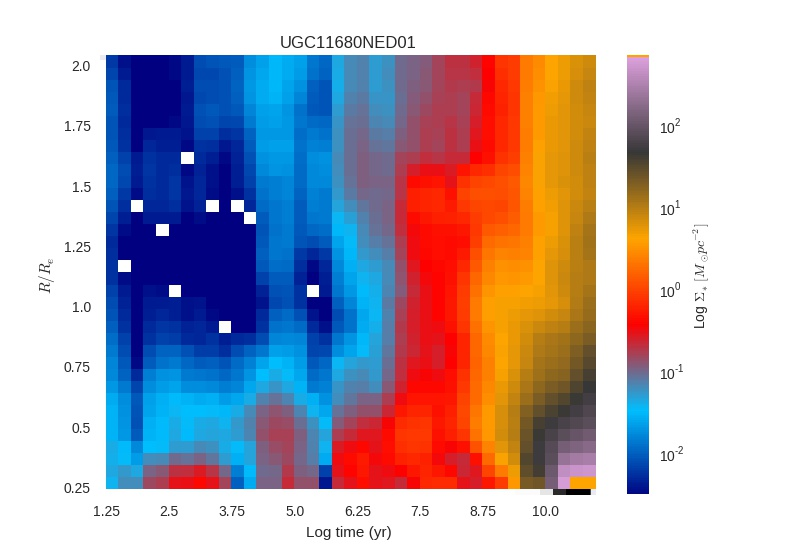
\includegraphics[width=.45\linewidth] {03_GraphicFiles/figure_1.jpg}   
\label{fig:subfig1} }
\end{subfigure}
\hfill
% -------------- SUBFIGURE -2 -------------- %
\begin{subfigure}{
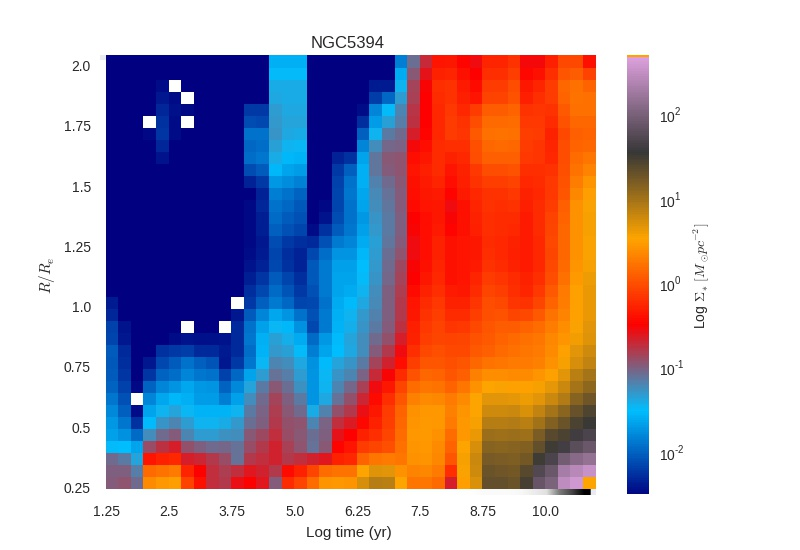
\includegraphics[width=.45\linewidth] {03_GraphicFiles/figure_2.jpg}
\label{fig:subfig2} }%
\end{subfigure}
\hfill
% -------------- SUBFIGURE -3 -------------- %
\begin{subfigure}{
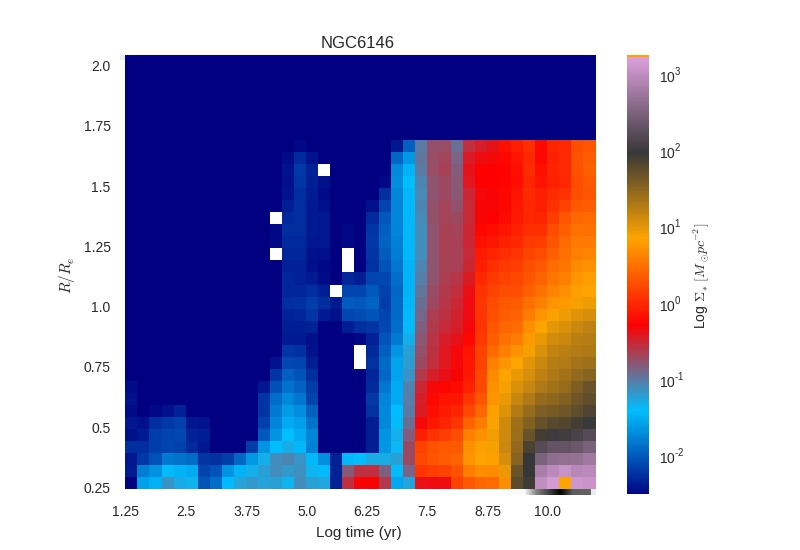
\includegraphics[width=.45\linewidth] {03_GraphicFiles/figure_3.jpg}
\label{fig:subfig3} }%
\end{subfigure}%
\hfill
% --------------SUBFIGURE -4 -------------- %
\begin{subfigure}{
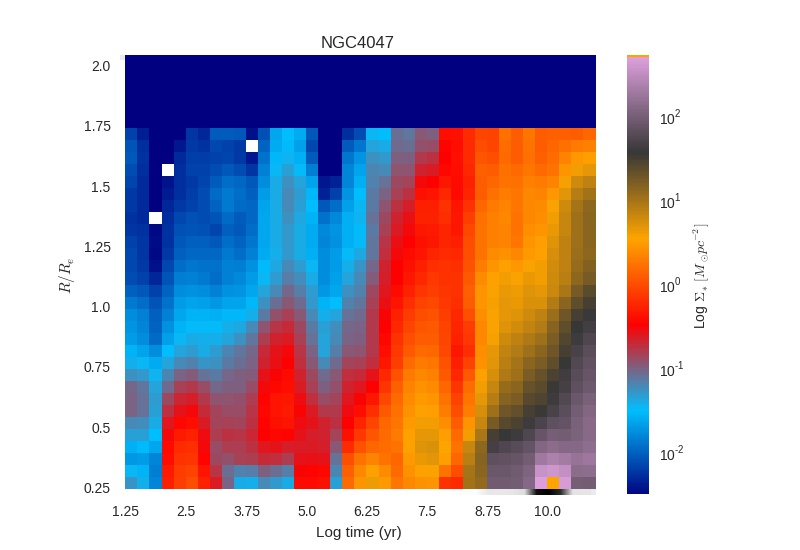
\includegraphics[width=.45\linewidth] {03_GraphicFiles/figure_4.jpg}
\label{fig:subfig4} }%
\end{subfigure}%
 
\label{myfigure}                            % label to the whole figure
\caption{Four Historiograms for different galaxies:UGC11680NED01,the red spiral. NGC5394,a interacting starburst galaxy.NGC6146,a typical elliptical 
galaxy and NGC4047,a face-on blue spiral.}
\end{figure}



\chapter{Dude (looks like an AGN)}


\begin{figure}[H]
\centering
	\includegraphics[width=1\textwidth]%
	{03_GraphicFiles/figure_14.png}%
\caption[A cow]{Color-Mass Diagram for the CALIFA survey. Each bin includes the mass assembly history tracks for different effective radius (nucleus,
middle range and outskirts) The time scale is linear. Notice the inside-out grow in stellar mass. }
\label{fig:14}
\end{figure}


\begin{figure}[H]
\centering
	\includegraphics[width=1\textwidth]%
	{03_GraphicFiles/figure_15.jpg}%
\caption[A cow]{Color-Mass Diagram for the CALIFA survey. Each bin includes the mass assembly history tracks for different effective radius (nucleus,
middle range and outskirts) The time scale is logarithmic. Notice the inside-out grow in stellar mass. }
\label{fig:15}
\end{figure}




\chapter{The $\chi^2$ Measure}

For a > 0, the gamma function G(a) is defined by


The most important properties of the gamma function are the following:

A continuous random variable X is said to have a gamma distribution if the
pdf of X is

Figure 4.26(a) illustrates the graphs of the gamma pdf for several (a, b) pairs, whereas
Figure 4.26(b) presents graphs of the standard gamma pdf. For the standard pdf,
when a 1, f(x; a) is strictly decreasing as x increases; when a > 1, f(x; a) rises to a maximum and then decreases. The parameter b in (4.7) is called the scale parameter
because values other than 1 either stretch or compress the pdf in the x direction.


DEFINITION Let n be a positive integer. Then a random variable X is said to have a chi squared distribution with parameter n if the pdf of X is the gamma density with a 1?4 n/2 and b 1?4 2. The pdf of a chi-squared rv is thus

The chi-squared distribution is important because it is the basis for a number
of procedures in statistical inference. The reason for this is that chi-squared
distributions are intimately related to normal distributions




\begin{figure}[!ht]
\centering
% -------------- SUBFIGURE -1 -------------- %
\begin{subfigure}{
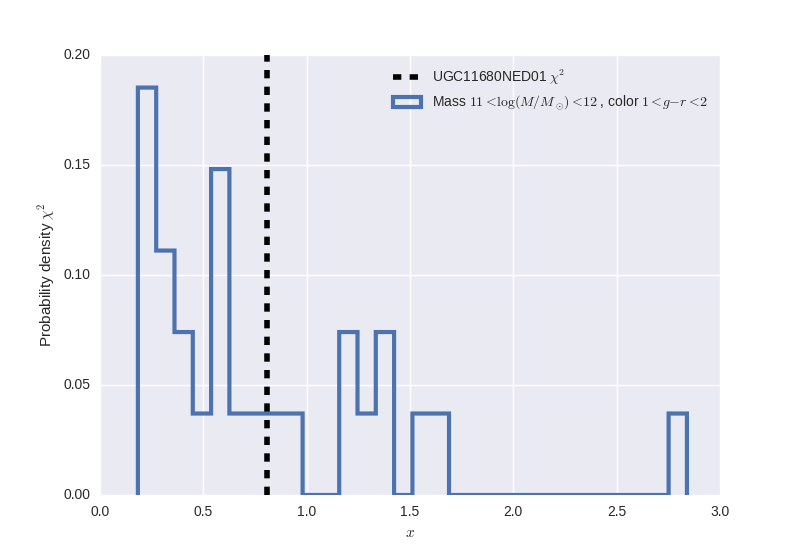
\includegraphics[width=.45\linewidth] {03_GraphicFiles/figure_27.png}   
\label{fig:subfig27} }
\end{subfigure}
\hfill
% -------------- SUBFIGURE -2 -------------- %
\begin{subfigure}{
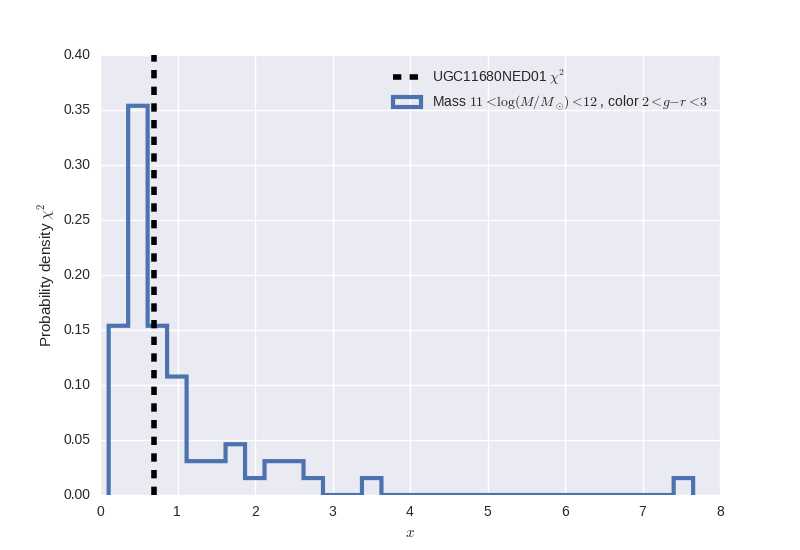
\includegraphics[width=.45\linewidth] {03_GraphicFiles/figure_26.png}
\label{fig:subfig28} }%
\end{subfigure}
\hfill
% -------------- SUBFIGURE -3 -------------- %
\begin{subfigure}{
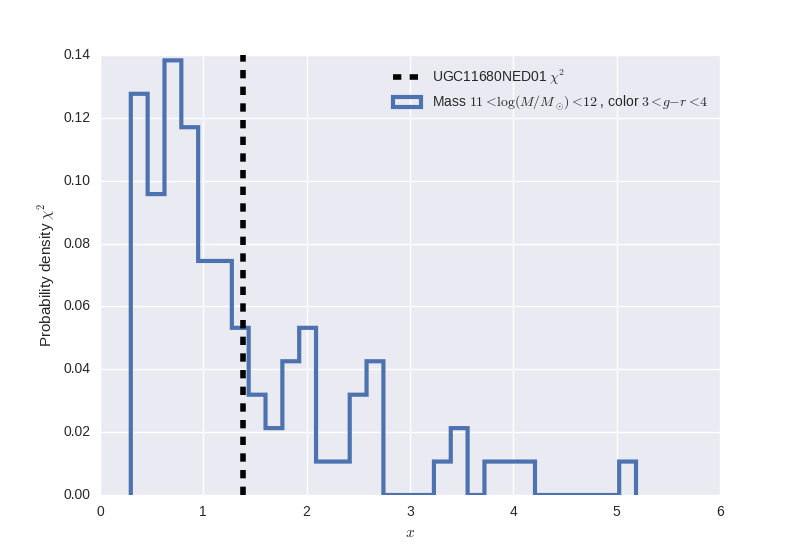
\includegraphics[width=.45\linewidth] {03_GraphicFiles/figure_24.png}
\label{fig:subfig29} }%
\end{subfigure}%
\hfill
% --------------SUBFIGURE -4 -------------- %
\begin{subfigure}{
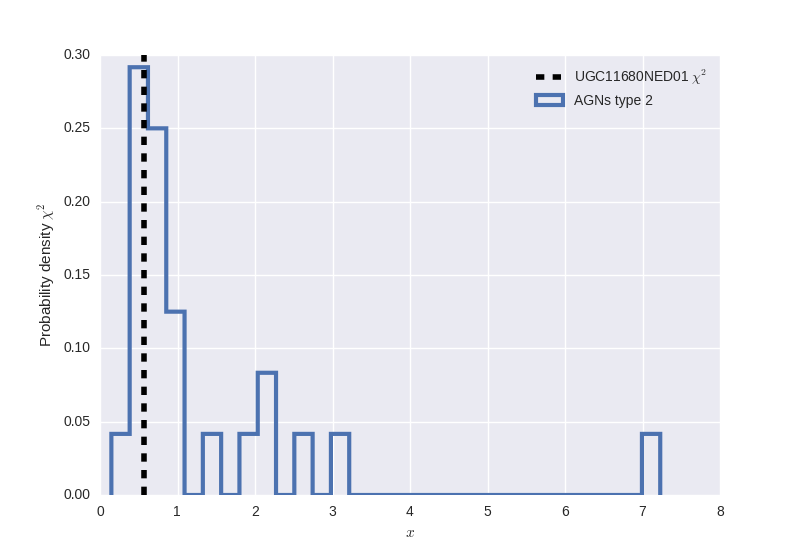
\includegraphics[width=.45\linewidth] {03_GraphicFiles/figure_32.png}
\label{fig:subfig30} }%
\end{subfigure}%


 
\label{myfigure}                            % label to the whole figure
\caption{$\chi^2$ reducided distribution for all galaxies in the mass range $11<\log (M/M_{\odot})<12$  in the CALIFA survey, subdivided by color $g-r$ bins. The Black dashed line represents
the $\chi^2$ reducided value of UGC11680NED01 compared with each mass bin average. The bootom-right figure is the all AGNS $\chi^2$ reducided distribution}
\end{figure}





\begin{figure}[!ht]
\centering
% -------------- SUBFIGURE -1 -------------- %
\begin{subfigure}{
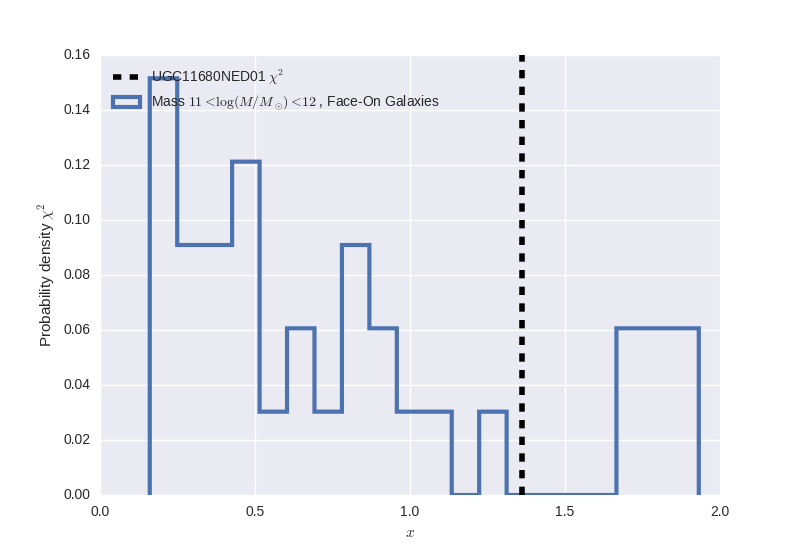
\includegraphics[width=.45\linewidth] {03_GraphicFiles/figure_34.png}   
\label{fig:subfig34} }
\end{subfigure}
\hfill
% -------------- SUBFIGURE -2 -------------- %
\begin{subfigure}{
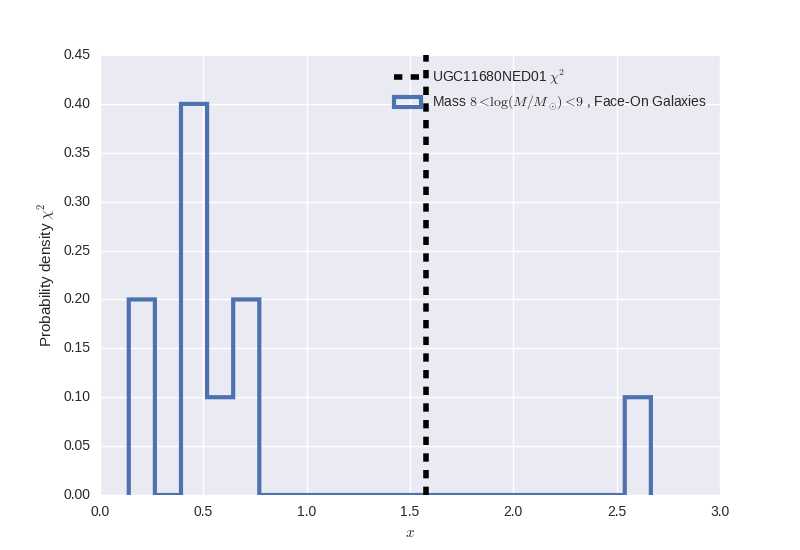
\includegraphics[width=.45\linewidth] {03_GraphicFiles/figure_35.png}
\label{fig:subfig35} }%
\end{subfigure}
\hfill
% -------------- SUBFIGURE -3 -------------- %
\begin{subfigure}{
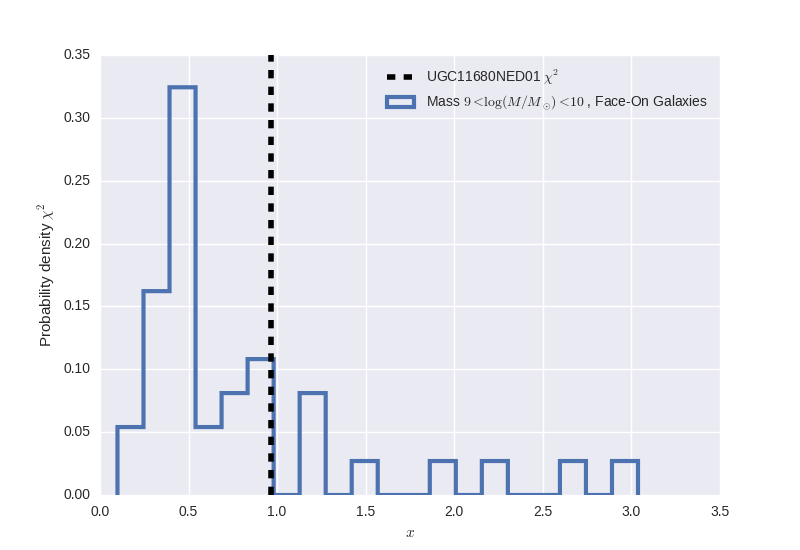
\includegraphics[width=.45\linewidth] {03_GraphicFiles/figure_37.png}
\label{fig:subfig37} }%
\end{subfigure}%
\hfill
% --------------SUBFIGURE -4 -------------- %
\begin{subfigure}{
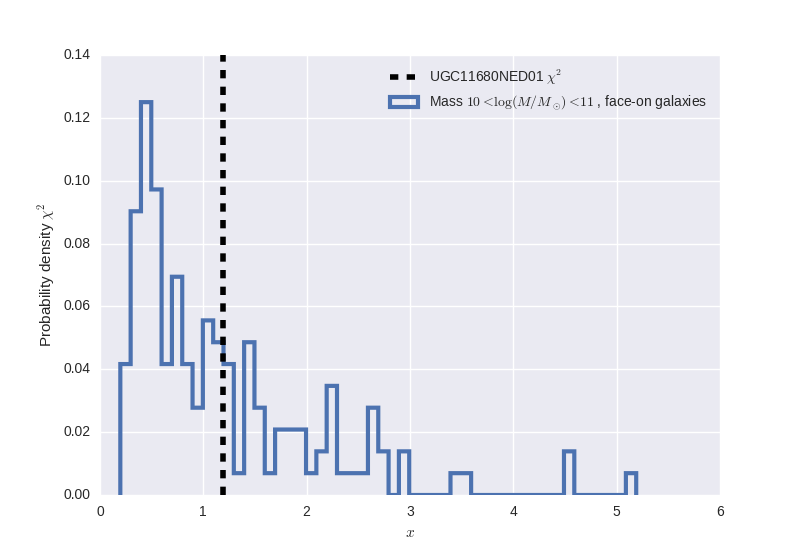
\includegraphics[width=.45\linewidth] {03_GraphicFiles/figure_38.png}
\label{fig:subfig38} }%
\end{subfigure}%
 
\label{myfigure}                            % label to the whole figure
\caption{$\chi^2$ reducided distribution for all Face-On Spiral Galaxies in the CALIFA survey, subdivided in mass bins. The Black dashed line represents
the $\chi^2$ reducided value of UGC11680NED01 compared with each mass bin average}
\end{figure}





% Final Thoughts
%%% File encoding is ISO-8859-1 (also known as Latin-1)
%%% You can use special characters just like �,� and �

\chapter{Final Thoughts}

\Blindtext[2][1]

% Start appendix
\appendix

% Appendix A
%%% File encoding is ISO-8859-1 (also known as Latin-1)
%%% You can use special characters just like �,� and �

\chapter{Appendix Chapter}

\Blindtext[3][1]

\section{Appendix Section}

\Blindtext[2][2]

\subsection{Appendix Sub-Section}

\Blindtext[2][1]

% Appendix B
%%% File encoding is ISO-8859-1 (also known as Latin-1)
%%% You can use special characters just like �,� and �

\chapter{Another Appendix Chapter}

\blindtext

%\begin{thebibliography}


\expandafter\ifx\csname natexlab\endcsname\relax\def\natexlab#1{#1}\fi
\expandafter\ifx\csname href\endcsname\relax
  \def\href#1#2{}\fi
\expandafter\ifx\csname urllinklabel\endcsname\relax
  \def\urllinklabel{[LINK]}\fi
\expandafter\ifx\csname adsurllinklabel\endcsname\relax
  \def\adsurllinklabel{[ADS]}\fi

\bibitem[{Aaronson {et~al.}(1978)Aaronson, Cohen, Mould, \&
  Malkan}]{Aaronson:1978p3433}
Aaronson, M., Cohen, J.~G., Mould, J., \& Malkan, M. 1978, ApJ, 223, 824
 \href{http://adsabs.harvard.edu/cgi-bin/nph-data_query?bibcode=1978ApJ...223.%
.824A&link_type=ABSTRACT}{\urllinklabel}

\bibitem[{{Barrera-Ballesteros} {et~al.}(2014){Barrera-Ballesteros},
  {Falc{\'o}n-Barroso}, {Garc{\'{\i}}a-Lorenzo}, {van de Ven}, {Aguerri},
  {Mendez-Abreu}, {Spekkens}, {Lyubenova}, {S{\'a}nchez}, {Husemann}, {Mast},
  {Garc{\'{\i}}a-Benito}, {Iglesias-Paramo}, {Del Olmo}, {M{\'a}rquez},
  {Masegosa}, {Kehrig}, {Marino}, {Verdes-Montenegro}, {Ziegler}, {McIntosh},
  {Bland-Hawthorn}, {Walcher}, \& {Califa Collaboration}}]{jkbb14}
{Barrera-Ballesteros}, J.~K., {Falc{\'o}n-Barroso}, J.,
  {Garc{\'{\i}}a-Lorenzo}, B., {van de Ven}, G., {Aguerri}, J.~A.~L.,
  {Mendez-Abreu}, J., {Spekkens}, K., {Lyubenova}, M., {S{\'a}nchez}, S.~F.,
  {Husemann}, B., {Mast}, D., {Garc{\'{\i}}a-Benito}, R., {Iglesias-Paramo},
  J., {Del Olmo}, A., {M{\'a}rquez}, I., {Masegosa}, J., {Kehrig}, C.,
  {Marino}, R.~A., {Verdes-Montenegro}, L., {Ziegler}, B., {McIntosh}, D.~H.,
  {Bland-Hawthorn}, J., {Walcher}, C.~J., \& {Califa Collaboration}. 2014,
  \aap, 568, A70


\bibitem[{Bruzual \& Charlot(2003)}]{bc03}
Bruzual, G. \& Charlot, S. 2003, Mon. Not. R. Astron. Soc., 344, 1000
 \href{http://adsabs.harvard.edu/cgi-bin/nph-data_query?bibcode=2003MNRAS.344.%
1000B&link_type=ABSTRACT}{\urllinklabel}

\bibitem[{{Bundy} {et~al.}(2015){Bundy}, {Bershady}, {Law}, {Yan}, {Drory},
  {MacDonald}, {Wake}, {Cherinka}, {S{\'a}nchez-Gallego}, {Weijmans}, {Thomas},
  {Tremonti}, {Masters}, {Coccato}, {Diamond-Stanic}, {Arag{\'o}n-Salamanca},
  {Avila-Reese}, {Badenes}, {Falc{\'o}n-Barroso}, {Belfiore}, {Bizyaev},
  {Blanc}, {Bland-Hawthorn}, {Blanton}, {Brownstein}, {Byler}, {Cappellari},
  {Conroy}, {Dutton}, {Emsellem}, {Etherington}, {Frinchaboy}, {Fu}, {Gunn},
  {Harding}, {Johnston}, {Kauffmann}, {Kinemuchi}, {Klaene}, {Knapen},
  {Leauthaud}, {Li}, {Lin}, {Maiolino}, {Malanushenko}, {Malanushenko}, {Mao},
  {Maraston}, {McDermid}, {Merrifield}, {Nichol}, {Oravetz}, {Pan}, {Parejko},
  {Sanchez}, {Schlegel}, {Simmons}, {Steele}, {Steinmetz}, {Thanjavur},
  {Thompson}, {Tinker}, {van den Bosch}, {Westfall}, {Wilkinson}, {Wright},
  {Xiao}, \& {Zhang}}]{manga}
{Bundy}, K., {Bershady}, M.~A., {Law}, D.~R., {Yan}, R., {Drory}, N.,
  {MacDonald}, N., {Wake}, D.~A., {Cherinka}, B., {S{\'a}nchez-Gallego}, J.~R.,
  {Weijmans}, A.-M., {Thomas}, D., {Tremonti}, C., {Masters}, K., {Coccato},
  L., {Diamond-Stanic}, A.~M., {Arag{\'o}n-Salamanca}, A., {Avila-Reese}, V.,
  {Badenes}, C., {Falc{\'o}n-Barroso}, J., {Belfiore}, F., {Bizyaev}, D.,
  {Blanc}, G.~A., {Bland-Hawthorn}, J., {Blanton}, M.~R., {Brownstein}, J.~R.,
  {Byler}, N., {Cappellari}, M., {Conroy}, C., {Dutton}, A.~A., {Emsellem}, E.,
  {Etherington}, J., {Frinchaboy}, P.~M., {Fu}, H., {Gunn}, J.~E., {Harding},
  P., {Johnston}, E.~J., {Kauffmann}, G., {Kinemuchi}, K., {Klaene}, M.~A.,
  {Knapen}, J.~H., {Leauthaud}, A., {Li}, C., {Lin}, L., {Maiolino}, R.,
  {Malanushenko}, V., {Malanushenko}, E., {Mao}, S., {Maraston}, C.,
  {McDermid}, R.~M., {Merrifield}, M.~R., {Nichol}, R.~C., {Oravetz}, D.,
  {Pan}, K., {Parejko}, J.~K., {Sanchez}, S.~F., {Schlegel}, D., {Simmons}, A.,
  {Steele}, O., {Steinmetz}, M., {Thanjavur}, K., {Thompson}, B.~A., {Tinker},
  J.~L., {van den Bosch}, R.~C.~E., {Westfall}, K.~B., {Wilkinson}, D.,
  {Wright}, S., {Xiao}, T., \& {Zhang}, K. 2015, \apj, 798, 7


\bibitem[{{Calzetti}(2001)}]{calz01}
{Calzetti}, D. 2001, \pasp, 113, 1449


\bibitem[{{Cappellari} \& {Emsellem}(2004{\natexlab{a}})}]{cappe04}
{Cappellari}, M. \& {Emsellem}, E. 2004{\natexlab{a}}, \pasp, 116, 138


\bibitem[{{Cappellari} \& {Emsellem}(2004{\natexlab{b}})}]{cappellari04}
---. 2004{\natexlab{b}}, \pasp, 116, 138


\bibitem[{{Cardelli} {et~al.}(1989){Cardelli}, {Clayton}, \&
  {Mathis}}]{cardelli89}
{Cardelli}, J.~A., {Clayton}, G.~C., \& {Mathis}, J.~S. 1989, \apj, 345, 245


\bibitem[{Cardiel {et~al.}(2003)Cardiel, Gorgas, S{\'a}nchez-Bl{\'a}zquez,
  Cenarro, Pedraz, Bruzual, \& Klement}]{Cardiel:2003p3435}
Cardiel, N., Gorgas, J., S{\'a}nchez-Bl{\'a}zquez, P., Cenarro, A.~J., Pedraz,
  S., Bruzual, G., \& Klement, J. 2003, A\&A, 409, 511
 \href{http://adsabs.harvard.edu/cgi-bin/nph-data_query?bibcode=2003A\%2526A..%
.409..511C&link_type=ABSTRACT}{\urllinklabel}

\bibitem[{Chabrier(2003)}]{Chabrier:2003p3777}
Chabrier, G. 2003, PASP, 115, 763
 \href{http://adsabs.harvard.edu/cgi-bin/nph-data_query?bibcode=2003PASP..115.%
.763C&link_type=ABSTRACT}{\urllinklabel}

\bibitem[{Charlot \& Fall(2000)}]{Charlot:2000p3439}
Charlot, S. \& Fall, S.~M. 2000, ApJ, 539, 718
 \href{http://adsabs.harvard.edu/cgi-bin/nph-data_query?bibcode=2000ApJ...539.%
.718C&link_type=ABSTRACT}{\urllinklabel}

\bibitem[{{Cid Fernandes} {et~al.}(2014){Cid Fernandes}, {Gonz{\'a}lez
  Delgado}, {Garc{\'{\i}}a Benito}, {P{\'e}rez}, {de Amorim}, {S{\'a}nchez},
  {Husemann}, {Falc{\'o}n Barroso}, {L{\'o}pez-Fern{\'a}ndez},
  {S{\'a}nchez-Bl{\'a}zquez}, {Vale Asari}, {Vazdekis}, {Walcher}, \&
  {Mast}}]{cid-fernandes14}
{Cid Fernandes}, R., {Gonz{\'a}lez Delgado}, R.~M., {Garc{\'{\i}}a Benito}, R.,
  {P{\'e}rez}, E., {de Amorim}, A.~L., {S{\'a}nchez}, S.~F., {Husemann}, B.,
  {Falc{\'o}n Barroso}, J., {L{\'o}pez-Fern{\'a}ndez}, R.,
  {S{\'a}nchez-Bl{\'a}zquez}, P., {Vale Asari}, N., {Vazdekis}, A., {Walcher},
  C.~J., \& {Mast}, D. 2014, \aap, 561, A130


\bibitem[{{Cid Fernandes} {et~al.}(2005){Cid Fernandes}, {Mateus}, {Sodr{\'e}},
  {Stasi{\'n}ska}, \& {Gomes}}]{cid-fernandes05}
{Cid Fernandes}, R., {Mateus}, A., {Sodr{\'e}}, L., {Stasi{\'n}ska}, G., \&
  {Gomes}, J.~M. 2005, \mnras, 358, 363


\bibitem[{{Cid Fernandes} {et~al.}(2013){Cid Fernandes}, {P{\'e}rez},
  {Garc{\'{\i}}a Benito}, {Gonz{\'a}lez Delgado}, {de Amorim}, {S{\'a}nchez},
  {Husemann}, {Falc{\'o}n Barroso}, {S{\'a}nchez-Bl{\'a}zquez}, {Walcher}, \&
  {Mast}}]{cid-fernandes13}
{Cid Fernandes}, R., {P{\'e}rez}, E., {Garc{\'{\i}}a Benito}, R., {Gonz{\'a}lez
  Delgado}, R.~M., {de Amorim}, A.~L., {S{\'a}nchez}, S.~F., {Husemann}, B.,
  {Falc{\'o}n Barroso}, J., {S{\'a}nchez-Bl{\'a}zquez}, P., {Walcher}, C.~J.,
  \& {Mast}, D. 2013, \aap, 557, A86


\bibitem[{{Courteau} {et~al.}(2014){Courteau}, {Cappellari}, {de Jong},
  {Dutton}, {Emsellem}, {Hoekstra}, {Koopmans}, {Mamon}, {Maraston}, {Treu}, \&
  {Widrow}}]{court13}
{Courteau}, S., {Cappellari}, M., {de Jong}, R.~S., {Dutton}, A.~A.,
  {Emsellem}, E., {Hoekstra}, H., {Koopmans}, L.~V.~E., {Mamon}, G.~A.,
  {Maraston}, C., {Treu}, T., \& {Widrow}, L.~M. 2014, Reviews of Modern
  Physics, 86, 47


\bibitem[{{Croom} {et~al.}(2012){Croom}, {Lawrence}, {Bland-Hawthorn},
  {Bryant}, {Fogarty}, {Richards}, {Goodwin}, {Farrell}, {Miziarski}, {Heald},
  {Jones}, {Lee}, {Colless}, {Brough}, {Hopkins}, {Bauer}, {Birchall}, {Ellis},
  {Horton}, {Leon-Saval}, {Lewis}, {L{\'o}pez-S{\'a}nchez}, {Min}, {Trinh}, \&
  {Trowland}}]{sami}
{Croom}, S.~M., {Lawrence}, J.~S., {Bland-Hawthorn}, J., {Bryant}, J.~J.,
  {Fogarty}, L., {Richards}, S., {Goodwin}, M., {Farrell}, T., {Miziarski}, S.,
  {Heald}, R., {Jones}, D.~H., {Lee}, S., {Colless}, M., {Brough}, S.,
  {Hopkins}, A.~M., {Bauer}, A.~E., {Birchall}, M.~N., {Ellis}, S., {Horton},
  A., {Leon-Saval}, S., {Lewis}, G., {L{\'o}pez-S{\'a}nchez}, {\'A}.~R., {Min},
  S.-S., {Trinh}, C., \& {Trowland}, H. 2012, \mnras, 421, 872


\bibitem[{{Falc{\'o}n-Barroso} {et~al.}(2011){Falc{\'o}n-Barroso},
  {S{\'a}nchez-Bl{\'a}zquez}, {Vazdekis}, {Ricciardelli}, {Cardiel}, {Cenarro},
  {Gorgas}, \& {Peletier}}]{falc11}
{Falc{\'o}n-Barroso}, J., {S{\'a}nchez-Bl{\'a}zquez}, P., {Vazdekis}, A.,
  {Ricciardelli}, E., {Cardiel}, N., {Cenarro}, A.~J., {Gorgas}, J., \&
  {Peletier}, R.~F. 2011, \aap, 532, A95


\bibitem[{{Gerhard}(2003)}]{gerh2003}
{Gerhard}, O. in , The Mass of Galaxies at Low and High Redshift, ed.
  R.~{Bender}A.~{Renzini}, 62


\bibitem[{{Gil de Paz} \& {Madore}(2002)}]{gildepaz02}
{Gil de Paz}, A. \& {Madore}, B.~F. 2002, \aj, 123, 1864


\bibitem[{{Gonz{\'a}lez Delgado} {et~al.}(2005){Gonz{\'a}lez Delgado},
  {Cervi{\~n}o}, {Martins}, {Leitherer}, \& {Hauschildt}}]{rosa2005}
{Gonz{\'a}lez Delgado}, R.~M., {Cervi{\~n}o}, M., {Martins}, L.~P.,
  {Leitherer}, C., \& {Hauschildt}, P.~H. 2005, \mnras, 357, 945


\bibitem[{{Gonz{\'a}lez Delgado} {et~al.}(2015){Gonz{\'a}lez Delgado},
  {Garc{\'{\i}}a-Benito}, {P{\'e}rez}, {Cid Fernandes}, {de Amorim},
  {Cortijo-Ferrero}, {Lacerda}, {L{\'o}pez Fern{\'a}ndez}, {Vale-Asari},
  {S{\'a}nchez}, {Moll{\'a}}, {Ruiz-Lara}, {S{\'a}nchez-Bl{\'a}zquez},
  {Walcher}, {Alves}, {Aguerri}, {Bekerait{\'e}}, {Bland-Hawthorn}, {Galbany},
  {Gallazzi}, {Husemann}, {Iglesias-P{\'a}ramo}, {Kalinova},
  {L{\'o}pez-S{\'a}nchez}, {Marino}, {M{\'a}rquez}, {Masegosa}, {Mast},
  {M{\'e}ndez-Abreu}, {Mendoza}, {del Olmo}, {P{\'e}rez}, {Quirrenbach},
  {Zibetti}, \& {CALIFA collaboration}}]{rosa15a}
{Gonz{\'a}lez Delgado}, R.~M., {Garc{\'{\i}}a-Benito}, R., {P{\'e}rez}, E.,
  {Cid Fernandes}, R., {de Amorim}, A.~L., {Cortijo-Ferrero}, C., {Lacerda},
  E.~A.~D., {L{\'o}pez Fern{\'a}ndez}, R., {Vale-Asari}, N., {S{\'a}nchez},
  S.~F., {Moll{\'a}}, M., {Ruiz-Lara}, T., {S{\'a}nchez-Bl{\'a}zquez}, P.,
  {Walcher}, C.~J., {Alves}, J., {Aguerri}, J.~A.~L., {Bekerait{\'e}}, S.,
  {Bland-Hawthorn}, J., {Galbany}, L., {Gallazzi}, A., {Husemann}, B.,
  {Iglesias-P{\'a}ramo}, J., {Kalinova}, V., {L{\'o}pez-S{\'a}nchez}, A.~R.,
  {Marino}, R.~A., {M{\'a}rquez}, I., {Masegosa}, J., {Mast}, D.,
  {M{\'e}ndez-Abreu}, J., {Mendoza}, A., {del Olmo}, A., {P{\'e}rez}, I.,
  {Quirrenbach}, A., {Zibetti}, S., \& {CALIFA collaboration}. 2015, ArXiv
  e-prints


\bibitem[{{Gonz{\'a}lez Delgado} {et~al.}(2014){Gonz{\'a}lez Delgado},
  {P{\'e}rez}, {Cid Fernandes}, {Garc{\'{\i}}a-Benito}, {de Amorim},
  {S{\'a}nchez}, {Husemann}, {Cortijo-Ferrero}, {L{\'o}pez Fern{\'a}ndez},
  {S{\'a}nchez-Bl{\'a}zquez}, {Bekeraite}, {Walcher}, {Falc{\'o}n-Barroso},
  {Gallazzi}, {van de Ven}, {Alves}, {Bland-Hawthorn}, {Kennicutt}, {Kupko},
  {Lyubenova}, {Mast}, {Moll{\'a}}, {Marino}, {Quirrenbach}, {V{\'{\i}}lchez},
  \& {Wisotzki}}]{rosa14}
{Gonz{\'a}lez Delgado}, R.~M., {P{\'e}rez}, E., {Cid Fernandes}, R.,
  {Garc{\'{\i}}a-Benito}, R., {de Amorim}, A.~L., {S{\'a}nchez}, S.~F.,
  {Husemann}, B., {Cortijo-Ferrero}, C., {L{\'o}pez Fern{\'a}ndez}, R.,
  {S{\'a}nchez-Bl{\'a}zquez}, P., {Bekeraite}, S., {Walcher}, C.~J.,
  {Falc{\'o}n-Barroso}, J., {Gallazzi}, A., {van de Ven}, G., {Alves}, J.,
  {Bland-Hawthorn}, J., {Kennicutt}, R.~C., {Kupko}, D., {Lyubenova}, M.,
  {Mast}, D., {Moll{\'a}}, M., {Marino}, R.~A., {Quirrenbach}, A.,
  {V{\'{\i}}lchez}, J.~M., \& {Wisotzki}, L. 2014, \aap, 562, A47


\bibitem[{{Koleva} {et~al.}(2009){Koleva}, {Prugniel}, {Bouchard}, \&
  {Wu}}]{koleva2009}
{Koleva}, M., {Prugniel}, P., {Bouchard}, A., \& {Wu}, Y. 2009, \aap, 501, 1269


\bibitem[{{Le Borgne} {et~al.}(2003){Le Borgne}, {Bruzual}, {Pell{\'o}},
  {Lan{\c c}on}, {Rocca-Volmerange}, {Sanahuja}, {Schaerer}, {Soubiran}, \&
  {V{\'{\i}}lchez-G{\'o}mez}}]{stelib}
{Le Borgne}, J.-F., {Bruzual}, G., {Pell{\'o}}, R., {Lan{\c c}on}, A.,
  {Rocca-Volmerange}, B., {Sanahuja}, B., {Schaerer}, D., {Soubiran}, C., \&
  {V{\'{\i}}lchez-G{\'o}mez}, R. 2003, \aap, 402, 433


\bibitem[{{MacArthur} {et~al.}(2004){MacArthur}, {Courteau}, {Bell}, \&
  {Holtzman}}]{macarthur+04}
{MacArthur}, L.~A., {Courteau}, S., {Bell}, E., \& {Holtzman}, J.~A. 2004,
  \apjs, 152, 175


\bibitem[{{MacArthur} {et~al.}(2009){MacArthur}, {Gonz{\'a}lez}, \&
  {Courteau}}]{macarthur2009}
{MacArthur}, L.~A., {Gonz{\'a}lez}, J.~J., \& {Courteau}, S. 2009, \mnras, 395,
  28


\bibitem[{{Maraston}(2005)}]{mar05}
{Maraston}, C. 2005, \mnras, 362, 799


\bibitem[{{Maraston} \& {Str{\"o}mb{\"a}ck}(2011)}]{mar11}
{Maraston}, C. \& {Str{\"o}mb{\"a}ck}, G. 2011, \mnras, 418, 2785


\bibitem[{{M{\'a}rmol-Queralt{\'o}} {et~al.}(2011){M{\'a}rmol-Queralt{\'o}},
  {S{\'a}nchez}, {Marino}, {Mast}, {Viironen}, {Gil de Paz},
  {Iglesias-P{\'a}ramo}, {Rosales-Ortega}, \& {Vilchez}}]{marmol-queralto11}
{M{\'a}rmol-Queralt{\'o}}, E., {S{\'a}nchez}, S.~F., {Marino}, R.~A., {Mast},
  D., {Viironen}, K., {Gil de Paz}, A., {Iglesias-P{\'a}ramo}, J.,
  {Rosales-Ortega}, F.~F., \& {Vilchez}, J.~M. 2011, \aap, 534, A8


\bibitem[{{Martins} {et~al.}(2005){Martins}, {Gonz{\'a}lez Delgado},
  {Leitherer}, {Cervi{\~n}o}, \& {Hauschildt}}]{martins05}
{Martins}, L.~P., {Gonz{\'a}lez Delgado}, R.~M., {Leitherer}, C.,
  {Cervi{\~n}o}, M., \& {Hauschildt}, P. 2005, \mnras, 358, 49


\bibitem[{Oconnell(1976)}]{Oconnell:1976p3432}
Oconnell, R.~W. 1976, ApJ, 206, 370
 \href{http://adsabs.harvard.edu/cgi-bin/nph-data_query?bibcode=1976ApJ...206.%
.370O&link_type=ABSTRACT}{\urllinklabel}

\bibitem[{{Ocvirk} {et~al.}(2006){Ocvirk}, {Pichon}, {Lan{\c c}on}, \&
  {Thi{\'e}baut}}]{ocvrik2006}
{Ocvirk}, P., {Pichon}, C., {Lan{\c c}on}, A., \& {Thi{\'e}baut}, E. 2006,
  \mnras, 365, 46


\bibitem[{{Panter} {et~al.}(2003){Panter}, {Heavens}, \& {Jimenez}}]{pant2003}
{Panter}, B., {Heavens}, A.~F., \& {Jimenez}, R. 2003, \mnras, 343, 1145


\bibitem[{{Papaderos} {et~al.}(2013){Papaderos}, {Gomes}, {V{\'{\i}}lchez},
  {Kehrig}, {Lehnert}, {Ziegler}, {S{\'a}nchez}, {Husemann}, {Monreal-Ibero},
  {Garc{\'{\i}}a-Benito}, {Bland-Hawthorn}, {Cortijo-Ferrero}, {de
  Lorenzo-C{\'a}ceres}, {del Olmo}, {Falc{\'o}n-Barroso}, {Galbany},
  {Iglesias-P{\'a}ramo}, {L{\'o}pez-S{\'a}nchez}, {Marquez}, {Moll{\'a}},
  {Mast}, {van de Ven}, \& {Wisotzki}}]{papa13}
{Papaderos}, P., {Gomes}, J.~M., {V{\'{\i}}lchez}, J.~M., {Kehrig}, C.,
  {Lehnert}, M.~D., {Ziegler}, B., {S{\'a}nchez}, S.~F., {Husemann}, B.,
  {Monreal-Ibero}, A., {Garc{\'{\i}}a-Benito}, R., {Bland-Hawthorn}, J.,
  {Cortijo-Ferrero}, C., {de Lorenzo-C{\'a}ceres}, A., {del Olmo}, A.,
  {Falc{\'o}n-Barroso}, J., {Galbany}, L., {Iglesias-P{\'a}ramo}, J.,
  {L{\'o}pez-S{\'a}nchez}, {\'A}.~R., {Marquez}, I., {Moll{\'a}}, M., {Mast},
  D., {van de Ven}, G., \& {Wisotzki}, L. 2013, \aap, 555, L1


\bibitem[{{P{\'e}rez} {et~al.}(2013){P{\'e}rez}, {Cid Fernandes}, {Gonz{\'a}lez
  Delgado}, {Garc{\'{\i}}a-Benito}, {S{\'a}nchez}, {Husemann}, {Mast},
  {Rod{\'o}n}, {Kupko}, {Backsmann}, {de Amorim}, {van de Ven}, {Walcher},
  {Wisotzki}, {Cortijo-Ferrero}, \& {CALIFA Collaboration}}]{eperez13}
{P{\'e}rez}, E., {Cid Fernandes}, R., {Gonz{\'a}lez Delgado}, R.~M.,
  {Garc{\'{\i}}a-Benito}, R., {S{\'a}nchez}, S.~F., {Husemann}, B., {Mast}, D.,
  {Rod{\'o}n}, J.~R., {Kupko}, D., {Backsmann}, N., {de Amorim}, A.~L., {van de
  Ven}, G., {Walcher}, J., {Wisotzki}, L., {Cortijo-Ferrero}, C., \& {CALIFA
  Collaboration}. 2013, \apjl, 764, L1


\bibitem[{{Rix} \& {White}(1992)}]{rix92}
{Rix}, H.-W. \& {White}, S.~D.~M. 1992, \mnras, 254, 389


\bibitem[{{Rosales-Ortega} {et~al.}(2010){Rosales-Ortega}, {Kennicutt},
  {S{\'a}nchez}, {D{\'{\i}}az}, {Pasquali}, {Johnson}, \&
  {Hao}}]{rosales-ortega10}
{Rosales-Ortega}, F.~F., {Kennicutt}, R.~C., {S{\'a}nchez}, S.~F.,
  {D{\'{\i}}az}, A.~I., {Pasquali}, A., {Johnson}, B.~D., \& {Hao}, C.~N. 2010,
  \mnras, 405, 735


\bibitem[{Salpeter(1955)}]{Salpeter:1955p3438}
Salpeter, E.~E. 1955, ApJ, 121, 161
 \href{http://adsabs.harvard.edu/cgi-bin/nph-data_query?bibcode=1955ApJ...121.%
.161S&link_type=ABSTRACT}{\urllinklabel}

\bibitem[{{S{\'a}nchez}(2006a)}]{sanchez06a}
{S{\'a}nchez}, S.~F. 2006a, Astronomische Nachrichten, 327, 850


\bibitem[{{S{\'a}nchez} {et~al.}(2007a){S{\'a}nchez}, {Aceituno}, {Thiele},
  {P{\'e}rez-Ram{\'{\i}}rez}, \& {Alves}}]{sanchez07a}
{S{\'a}nchez}, S.~F., {Aceituno}, J., {Thiele}, U., {P{\'e}rez-Ram{\'{\i}}rez},
  D., \& {Alves}, J. 2007a, \pasp, 119, 1186


\bibitem[{{S{\'a}nchez} {et~al.}(2007b){S{\'a}nchez}, {Cardiel}, {Verheijen},
  {Pedraz}, \& {Covone}}]{sanchez07b}
{S{\'a}nchez}, S.~F., {Cardiel}, N., {Verheijen}, M.~A.~W., {Pedraz}, S., \&
  {Covone}, G. 2007b, \mnras, 376, 125


\bibitem[{{S{\'a}nchez} {et~al.}(2006b){S{\'a}nchez}, {Garc{\'{\i}}a-Lorenzo},
  {Jahnke}, {Mediavilla}, {Gonz{\'a}lez-Serrano}, {Christensen}, \&
  {Wisotzki}}]{sanchez06b}
{S{\'a}nchez}, S.~F., {Garc{\'{\i}}a-Lorenzo}, B., {Jahnke}, K., {Mediavilla},
  E., {Gonz{\'a}lez-Serrano}, J.~I., {Christensen}, L., \& {Wisotzki}, L.
  2006b, \nar, 49, 501


\bibitem[{{S{\'a}nchez} {et~al.}(2012{\natexlab{a}}){S{\'a}nchez}, {Kennicutt},
  {Gil de Paz}, {van de Ven}, {V{\'{\i}}lchez}, {Wisotzki}, {Walcher}, {Mast},
  {Aguerri}, {Albiol-P{\'e}rez}, {Alonso-Herrero}, {Alves}, {Bakos},
  {Bart{\'a}kov{\'a}}, {Bland-Hawthorn}, {Boselli}, {Bomans},
  {Castillo-Morales}, {Cortijo-Ferrero}, {de Lorenzo-C{\'a}ceres}, {Del Olmo},
  {Dettmar}, {D{\'{\i}}az}, {Ellis}, {Falc{\'o}n-Barroso}, {Flores},
  {Gallazzi}, {Garc{\'{\i}}a-Lorenzo}, {Gonz{\'a}lez Delgado}, {Gruel},
  {Haines}, {Hao}, {Husemann}, {Igl{\'e}sias-P{\'a}ramo}, {Jahnke}, {Johnson},
  {Jungwiert}, {Kalinova}, {Kehrig}, {Kupko}, {L{\'o}pez-S{\'a}nchez},
  {Lyubenova}, {Marino}, {M{\'a}rmol-Queralt{\'o}}, {M{\'a}rquez}, {Masegosa},
  {Meidt}, {Mendez-Abreu}, {Monreal-Ibero}, {Montijo}, {Mour{\~a}o},
  {Palacios-Navarro}, {Papaderos}, {Pasquali}, {Peletier}, {P{\'e}rez},
  {P{\'e}rez}, {Quirrenbach}, {Rela{\~n}o}, {Rosales-Ortega}, {Roth},
  {Ruiz-Lara}, {S{\'a}nchez-Bl{\'a}zquez}, {Sengupta}, {Singh}, {Stanishev},
  {Trager}, {Vazdekis}, {Viironen}, {Wild}, {Zibetti}, \&
  {Ziegler}}]{sanchez12a}
{S{\'a}nchez}, S.~F., {Kennicutt}, R.~C., {Gil de Paz}, A., {van de Ven}, G.,
  {V{\'{\i}}lchez}, J.~M., {Wisotzki}, L., {Walcher}, C.~J., {Mast}, D.,
  {Aguerri}, J.~A.~L., {Albiol-P{\'e}rez}, S., {Alonso-Herrero}, A., {Alves},
  J., {Bakos}, J., {Bart{\'a}kov{\'a}}, T., {Bland-Hawthorn}, J., {Boselli},
  A., {Bomans}, D.~J., {Castillo-Morales}, A., {Cortijo-Ferrero}, C., {de
  Lorenzo-C{\'a}ceres}, A., {Del Olmo}, A., {Dettmar}, R.-J., {D{\'{\i}}az},
  A., {Ellis}, S., {Falc{\'o}n-Barroso}, J., {Flores}, H., {Gallazzi}, A.,
  {Garc{\'{\i}}a-Lorenzo}, B., {Gonz{\'a}lez Delgado}, R., {Gruel}, N.,
  {Haines}, T., {Hao}, C., {Husemann}, B., {Igl{\'e}sias-P{\'a}ramo}, J.,
  {Jahnke}, K., {Johnson}, B., {Jungwiert}, B., {Kalinova}, V., {Kehrig}, C.,
  {Kupko}, D., {L{\'o}pez-S{\'a}nchez}, {\'A}.~R., {Lyubenova}, M., {Marino},
  R.~A., {M{\'a}rmol-Queralt{\'o}}, E., {M{\'a}rquez}, I., {Masegosa}, J.,
  {Meidt}, S., {Mendez-Abreu}, J., {Monreal-Ibero}, A., {Montijo}, C.,
  {Mour{\~a}o}, A.~M., {Palacios-Navarro}, G., {Papaderos}, P., {Pasquali}, A.,
  {Peletier}, R., {P{\'e}rez}, E., {P{\'e}rez}, I., {Quirrenbach}, A.,
  {Rela{\~n}o}, M., {Rosales-Ortega}, F.~F., {Roth}, M.~M., {Ruiz-Lara}, T.,
  {S{\'a}nchez-Bl{\'a}zquez}, P., {Sengupta}, C., {Singh}, R., {Stanishev}, V.,
  {Trager}, S.~C., {Vazdekis}, A., {Viironen}, K., {Wild}, V., {Zibetti}, S.,
  \& {Ziegler}, B. 2012{\natexlab{a}}, \aap, 538, A8


\bibitem[{{S{\'a}nchez} {et~al.}(2013){S{\'a}nchez}, {Rosales-Ortega},
  {Jungwiert}, {Iglesias-P{\'a}ramo}, {V{\'{\i}}lchez}, {Marino}, {Walcher},
  {Husemann}, {Mast}, {Monreal-Ibero}, {Cid Fernandes}, {P{\'e}rez},
  {Gonz{\'a}lez Delgado}, {Garc{\'{\i}}a-Benito}, {Galbany}, {van de Ven},
  {Jahnke}, {Flores}, {Bland-Hawthorn}, {L{\'o}pez-S{\'a}nchez}, {Stanishev},
  {Miralles-Caballero}, {D{\'{\i}}az}, {S{\'a}nchez-Blazquez}, {Moll{\'a}},
  {Gallazzi}, {Papaderos}, {Gomes}, {Gruel}, {P{\'e}rez}, {Ruiz-Lara},
  {Florido}, {de Lorenzo-C{\'a}ceres}, {Mendez-Abreu}, {Kehrig}, {Roth},
  {Ziegler}, {Alves}, {Wisotzki}, {Kupko}, {Quirrenbach}, {Bomans}, \& {Califa
  Collaboration}}]{sanchez13}
{S{\'a}nchez}, S.~F., {Rosales-Ortega}, F.~F., {Jungwiert}, B.,
  {Iglesias-P{\'a}ramo}, J., {V{\'{\i}}lchez}, J.~M., {Marino}, R.~A.,
  {Walcher}, C.~J., {Husemann}, B., {Mast}, D., {Monreal-Ibero}, A., {Cid
  Fernandes}, R., {P{\'e}rez}, E., {Gonz{\'a}lez Delgado}, R.,
  {Garc{\'{\i}}a-Benito}, R., {Galbany}, L., {van de Ven}, G., {Jahnke}, K.,
  {Flores}, H., {Bland-Hawthorn}, J., {L{\'o}pez-S{\'a}nchez}, A.~R.,
  {Stanishev}, V., {Miralles-Caballero}, D., {D{\'{\i}}az}, A.~I.,
  {S{\'a}nchez-Blazquez}, P., {Moll{\'a}}, M., {Gallazzi}, A., {Papaderos}, P.,
  {Gomes}, J.~M., {Gruel}, N., {P{\'e}rez}, I., {Ruiz-Lara}, T., {Florido}, E.,
  {de Lorenzo-C{\'a}ceres}, A., {Mendez-Abreu}, J., {Kehrig}, C., {Roth},
  M.~M., {Ziegler}, B., {Alves}, J., {Wisotzki}, L., {Kupko}, D.,
  {Quirrenbach}, A., {Bomans}, D., \& {Califa Collaboration}. 2013, \aap, 554,
  A58


\bibitem[{{S{\'a}nchez} {et~al.}(2011){S{\'a}nchez}, {Rosales-Ortega},
  {Kennicutt}, {Johnson}, {Diaz}, {Pasquali}, \& {Hao}}]{sanchez11}
{S{\'a}nchez}, S.~F., {Rosales-Ortega}, F.~F., {Kennicutt}, R.~C., {Johnson},
  B.~D., {Diaz}, A.~I., {Pasquali}, A., \& {Hao}, C.~N. 2011, \mnras, 410, 313


\bibitem[{{S{\'a}nchez} {et~al.}(2012{\natexlab{b}}){S{\'a}nchez},
  {Rosales-Ortega}, {Marino}, {Iglesias-P{\'a}ramo}, {V{\'{\i}}lchez},
  {Kennicutt}, {D{\'{\i}}az}, {Mast}, {Monreal-Ibero}, {Garc{\'{\i}}a-Benito},
  {Bland-Hawthorn}, {P{\'e}rez}, {Gonz{\'a}lez Delgado}, {Husemann},
  {L{\'o}pez-S{\'a}nchez}, {Cid Fernandes}, {Kehrig}, {Walcher}, {Gil de Paz},
  \& {Ellis}}]{sanchez12b}
{S{\'a}nchez}, S.~F., {Rosales-Ortega}, F.~F., {Marino}, R.~A.,
  {Iglesias-P{\'a}ramo}, J., {V{\'{\i}}lchez}, J.~M., {Kennicutt}, R.~C.,
  {D{\'{\i}}az}, A.~I., {Mast}, D., {Monreal-Ibero}, A.,
  {Garc{\'{\i}}a-Benito}, R., {Bland-Hawthorn}, J., {P{\'e}rez}, E.,
  {Gonz{\'a}lez Delgado}, R., {Husemann}, B., {L{\'o}pez-S{\'a}nchez},
  {\'A}.~R., {Cid Fernandes}, R., {Kehrig}, C., {Walcher}, C.~J., {Gil de Paz},
  A., \& {Ellis}, S. 2012{\natexlab{b}}, \aap, 546, A2


\bibitem[{{S{\'a}nchez-Bl{\'a}zquez} {et~al.}(2011){S{\'a}nchez-Bl{\'a}zquez},
  {Ocvirk}, {Gibson}, {P{\'e}rez}, \& {Peletier}}]{patri11}
{S{\'a}nchez-Bl{\'a}zquez}, P., {Ocvirk}, P., {Gibson}, B.~K., {P{\'e}rez}, I.,
  \& {Peletier}, R.~F. 2011, \mnras, 415, 709


\bibitem[{{S{\'a}nchez-Bl{\'a}zquez} {et~al.}(2006){S{\'a}nchez-Bl{\'a}zquez},
  {Peletier}, {Jim{\'e}nez-Vicente}, {Cardiel}, {Cenarro},
  {Falc{\'o}n-Barroso}, {Gorgas}, {Selam}, \& {Vazdekis}}]{miles}
{S{\'a}nchez-Bl{\'a}zquez}, P., {Peletier}, R.~F., {Jim{\'e}nez-Vicente}, J.,
  {Cardiel}, N., {Cenarro}, A.~J., {Falc{\'o}n-Barroso}, J., {Gorgas}, J.,
  {Selam}, S., \& {Vazdekis}, A. 2006, \mnras, 371, 703


\bibitem[{{S{\'a}nchez-Bl{\'a}zquez}
  {et~al.}(2014{\natexlab{a}}){S{\'a}nchez-Bl{\'a}zquez}, {Rosales-Ortega},
  {Diaz}, \& {S{\'a}nchez}}]{patri14a}
{S{\'a}nchez-Bl{\'a}zquez}, P., {Rosales-Ortega}, F., {Diaz}, A., \&
  {S{\'a}nchez}, S.~F. 2014{\natexlab{a}}, \mnras


\bibitem[{{S{\'a}nchez-Bl{\'a}zquez}
  {et~al.}(2014{\natexlab{b}}){S{\'a}nchez-Bl{\'a}zquez}, {Rosales-Ortega},
  {M{\'e}ndez-Abreu}, {P{\'e}rez}, {S{\'a}nchez}, {Zibetti}, {Aguerri},
  {Bland-Hawthorn}, {Catal{\'a}n-Torrecilla}, {Cid Fernandes}, {de Amorim}, {de
  Lorenzo-Caceres}, {Falc{\'o}n-Barroso}, {Galazzi}, {Garc{\'{\i}}a Benito},
  {Gil de Paz}, {Gonz{\'a}lez Delgado}, {Husemann}, {Iglesias-P{\'a}ramo},
  {Jungwiert}, {Marino}, {M{\'a}rquez}, {Mast}, {Mendoza}, {Moll{\'a}},
  {Papaderos}, {Ruiz-Lara}, {van de Ven}, {Walcher}, \& {Wisotzki}}]{patri14b}
{S{\'a}nchez-Bl{\'a}zquez}, P., {Rosales-Ortega}, F.~F., {M{\'e}ndez-Abreu},
  J., {P{\'e}rez}, I., {S{\'a}nchez}, S.~F., {Zibetti}, S., {Aguerri},
  J.~A.~L., {Bland-Hawthorn}, J., {Catal{\'a}n-Torrecilla}, C., {Cid
  Fernandes}, R., {de Amorim}, A., {de Lorenzo-Caceres}, A.,
  {Falc{\'o}n-Barroso}, J., {Galazzi}, A., {Garc{\'{\i}}a Benito}, R., {Gil de
  Paz}, A., {Gonz{\'a}lez Delgado}, R., {Husemann}, B., {Iglesias-P{\'a}ramo},
  J., {Jungwiert}, B., {Marino}, R.~A., {M{\'a}rquez}, I., {Mast}, D.,
  {Mendoza}, M.~A., {Moll{\'a}}, M., {Papaderos}, P., {Ruiz-Lara}, T., {van de
  Ven}, G., {Walcher}, C.~J., \& {Wisotzki}, L. 2014{\natexlab{b}}, \aap, 570,
  A6


\bibitem[{{Sarzi} {et~al.}(2006{\natexlab{a}}){Sarzi}, {Falc{\'o}n-Barroso},
  {Davies}, {Bacon}, {Bureau}, {Cappellari}, {de Zeeuw}, {Emsellem}, {Fathi},
  {Krajnovi{\'c}}, {Kuntschner}, {McDermid}, \& {Peletier}}]{sarzi2006}
{Sarzi}, M., {Falc{\'o}n-Barroso}, J., {Davies}, R.~L., {Bacon}, R., {Bureau},
  M., {Cappellari}, M., {de Zeeuw}, P.~T., {Emsellem}, E., {Fathi}, K.,
  {Krajnovi{\'c}}, D., {Kuntschner}, H., {McDermid}, R.~M., \& {Peletier},
  R.~F. 2006{\natexlab{a}}, \mnras, 366, 1151


\bibitem[{{Sarzi} {et~al.}(2006{\natexlab{b}}){Sarzi}, {Falc{\'o}n-Barroso},
  {Davies}, {Bacon}, {Bureau}, {Cappellari}, {de Zeeuw}, {Emsellem}, {Fathi},
  {Krajnovi{\'c}}, {Kuntschner}, {McDermid}, \& {Peletier}}]{sarzi06}
---. 2006{\natexlab{b}}, \mnras, 366, 1151


\bibitem[{{Serra} \& {Trager}(2007)}]{serra07}
{Serra}, P. \& {Trager}, S.~C. 2007, \mnras, 374, 769


\bibitem[{Stoklasov{\'a} {et~al.}(2009)Stoklasov{\'a}, Ferruit, Emsellem,
  Jungwiert, P{\'e}contal, \& S{\'a}nchez}]{Stoklasova:2009p3436}
Stoklasov{\'a}, I., Ferruit, P., Emsellem, E., Jungwiert, B., P{\'e}contal, E.,
  \& S{\'a}nchez, S.~F. 2009, A\&A, 500, 1287
 \href{http://adsabs.harvard.edu/cgi-bin/nph-data_query?bibcode=2009A\%2526A..%
.500.1287S&link_type=ABSTRACT}{\urllinklabel}

\bibitem[{Tinsley(1980)}]{Tinsley:1980p3431}
Tinsley, B.~M. 1980, FCPh, 5, 287
 \href{http://adsabs.harvard.edu/cgi-bin/nph-data_query?bibcode=1980FCPh....5.%
.287T&link_type=ABSTRACT}{\urllinklabel}

\bibitem[{{Tojeiro} {et~al.}(2007){Tojeiro}, {Heavens}, {Jimenez}, \&
  {Panter}}]{toje2007}
{Tojeiro}, R., {Heavens}, A.~F., {Jimenez}, R., \& {Panter}, B. 2007, \mnras,
  381, 1252


\bibitem[{{Tuffs} {et~al.}(2004){Tuffs}, {Popescu}, {V{\"o}lk}, {Kylafis}, \&
  {Dopita}}]{tuffs2004}
{Tuffs}, R.~J., {Popescu}, C.~C., {V{\"o}lk}, H.~J., {Kylafis}, N.~D., \&
  {Dopita}, M.~A. 2004, \aap, 419, 821


\bibitem[{{Vazdekis} {et~al.}(2010){Vazdekis}, {S{\'a}nchez-Bl{\'a}zquez},
  {Falc{\'o}n-Barroso}, {Cenarro}, {Beasley}, {Cardiel}, {Gorgas}, \&
  {Peletier}}]{vazdekis10}
{Vazdekis}, A., {S{\'a}nchez-Bl{\'a}zquez}, P., {Falc{\'o}n-Barroso}, J.,
  {Cenarro}, A.~J., {Beasley}, M.~A., {Cardiel}, N., {Gorgas}, J., \&
  {Peletier}, R.~F. 2010, \mnras, 404, 1639


\bibitem[{{Walcher} {et~al.}(2006){Walcher}, {B{\"o}ker}, {Charlot}, {Ho},
  {Rix}, {Rossa}, {Shields}, \& {van der Marel}}]{walch06}
{Walcher}, C.~J., {B{\"o}ker}, T., {Charlot}, S., {Ho}, L.~C., {Rix}, H.-W.,
  {Rossa}, J., {Shields}, J.~C., \& {van der Marel}, R.~P. 2006, \apj, 649, 692


\bibitem[{{Walcher} {et~al.}(2005){Walcher}, {van der Marel}, {McLaughlin},
  {Rix}, {B{\"o}ker}, {H{\"a}ring}, {Ho}, {Sarzi}, \& {Shields}}]{walcher05}
{Walcher}, C.~J., {van der Marel}, R.~P., {McLaughlin}, D., {Rix}, H.-W.,
  {B{\"o}ker}, T., {H{\"a}ring}, N., {Ho}, L.~C., {Sarzi}, M., \& {Shields},
  J.~C. 2005, \apj, 618, 237


\bibitem[{{Walcher} {et~al.}(2011){Walcher}, {Groves}, {Budav{\'a}ri}, \&
  {Dale}}]{walcher11}
{Walcher}, J., {Groves}, B., {Budav{\'a}ri}, T., \& {Dale}, D. 2011, \apss,
  331, 1


\bibitem[{{Wilkinson} {et~al.}(2015){Wilkinson}, {Maraston}, {Thomas},
  {Coccato}, {Tojeiro}, {Cappellari}, {Belfiore}, {Bershady}, {Blanton},
  {Bundy}, {Cales}, {Cherinka}, {Drory}, {Emsellem}, {Fu}, {Law}, {Li},
  {Maiolino}, {Masters}, {Tremonti}, {Wake}, {Wang}, {Weijmans}, {Xiao}, {Yan},
  {Zhang}, {Bizyaev}, {Brinkmann}, {Kinemuchi}, {Malanushenko}, {Malanushenko},
  {Oravetz}, {Pan}, \& {Simmons}}]{wilk15}
{Wilkinson}, D.~M., {Maraston}, C., {Thomas}, D., {Coccato}, L., {Tojeiro}, R.,
  {Cappellari}, M., {Belfiore}, F., {Bershady}, M., {Blanton}, M., {Bundy}, K.,
  {Cales}, S., {Cherinka}, B., {Drory}, N., {Emsellem}, E., {Fu}, H., {Law},
  D., {Li}, C., {Maiolino}, R., {Masters}, K., {Tremonti}, C., {Wake}, D.,
  {Wang}, E., {Weijmans}, A.-M., {Xiao}, T., {Yan}, R., {Zhang}, K., {Bizyaev},
  D., {Brinkmann}, J., {Kinemuchi}, K., {Malanushenko}, E., {Malanushenko}, V.,
  {Oravetz}, D., {Pan}, K., \& {Simmons}, A. 2015, \mnras, 449, 328


\bibitem[{Worthey(1994)}]{Worthey:1994p3434}
Worthey, G. 1994, ApJS, 95, 107
 \href{http://adsabs.harvard.edu/cgi-bin/nph-data_query?bibcode=1994ApJS...95.%
.107W&link_type=ABSTRACT}{\urllinklabel}

\end{thebibliography}

\end{document}
% ------------------------------------------------------------------
%
% #######################
% End: Document
% #######################
